\documentclass[a4paper,UKenglish,cleveref, autoref, thm-restate]{lipics-v2021}

%\documentclass[a4paper,UKenglish,cleveref, autoref, thm-restate]{lipics-v2021}
  % concur page limit: title + 15p + refs + 5p app
   
\usepackage{microtype}%if unwanted, comment out or use option "draft"
\usepackage{harengs}
\usepackage{ebproofs}
\usepackage{comment}
\usepackage{fge}
\usepackage{thm-restate}
\usepackage[new]{old-arrows}
\usepackage[utf8]{inputenc}
 \usepackage[all]{xy}
% \title{On graph homomorphisms and equational theories}
% \title{On graph homomorphisms, binary relations, and equational theories}
\title{Regular expressions for  tree-width 2 graphs}
\titlerunning{Regular expressions for tree-width 2 graphs}
\author{Anonymous}{Anonymous}{}{}{}

\authorrunning{Anonymous}
\Copyright{Anonymous}

%Editor-only macros:: begin (do not touch as author)%%%%%%%%%%%%%%%%%%%%%%%%%%%%%%%%%%
\EventEditors{John Q. Open and Joan R. Access}
\EventNoEds{2}
\EventLongTitle{42nd Conference on Very Important Topics (CVIT 2016)}
\EventShortTitle{CVIT 2016}
\EventAcronym{CVIT}
\EventYear{2016}
\EventDate{December 24--27, 2016}
\EventLocation{Little Whinging, United Kingdom}
\EventLogo{}
\SeriesVolume{42}
\ArticleNo{23}
%%%%%%%%%%%%%%%%%%%%%%%%%%%%%%%%%%%%%%%%%%%%%%%%%%%%%%

%\subjclass{F.3.1 Specifying, verifying, and reasoning about programs}
\keywords{Tree width, MSO, Regular expressions}
\ccsdesc[500]{Mathematics of computing~Discrete mathematics}
% \ccsdesc[500]{Theory of computation~Regular languages}
% \ccsdesc[500]{Theory of computation~Proof theory}

%\iflong
%\hideLIPIcs
%\DOIPrefix{}
%\renewcommand\copyrightline{}
%\nolinenumbers
%%\relatedversion{This is the full version of the paper with the same title published in Proc. CONCUR 2020, available at \url{https://doi.org/10.4230/LIPIcs.CONCUR.2020.49}}
%\else
%\nolinenumbers
%%\relatedversion{Appendix available at \url{https://hal.archives-ouvertes.fr/hal-02870687}}
%\fi

\begin{document}
\maketitle

\begin{abstract}
We propose a syntax of regular expressions, which describes languages of tree-width 2 graphs. We show that these languages correspond exactly to those languages of tree-width $2$ graphs, definable in the counting monadic second-order logic ($\CMSO$). 
\end{abstract}



%
\section{Introduction}

Regular word languages form a robust class of languages. One of the
witnesses for this robustness is the variety of equivalent formalisms defining them. They can be described by finite automata, by
monadic second-order ($\MSO$) formulas, by regular expressions or by finite
monoids~\cite{Buchi, Elgot, Kleene}. Each of these formalisms has some advantages, depending on the
context where it is used.
For example, $\MSO$ is close to natural language, regular expressions define regular languages via their closure properties, automata
have good algorithmic properties and can be used as actual algorithms to
decide membership in a language, etc. Similarly, regular tree languages have  equivalent formalisms, for various kinds of trees \cite{Kuske, Thatcher, Gcseg}.
\smallskip

We will here further generalize the structures considered, by moving to
graphs of bounded tree-width. Intuitively, they can be thought of as
``graphs which resemble trees''. In this framework, we already know that counting $\MSO$ ($\CMSO$), an extension of $\MSO$ with counting predicates, and recognizability by
algebra are equivalent \cite{BojanczykP16, BojanczykP17}, yielding a notion that
could be called ``regular languages of graphs of tree-width $k$''.
Engelfriet \cite{Engelfriet} also proposes a regular expressions formalism
matching this class, but by his own admission, these expressions closely
mimic the behavior of $\CMSO$. The main feature missing in Engelfriet's regular expressions is a mechanism for iteration, which is the central operator for word regular expressions: the Kleene star.
\smallskip

In this paper, we propose a syntax of regular expressions for languages
of tree-width $2$ graphs, that follow more closely the spirit of regular
expressions on words, using Kleene-like iterations.
This constitutes a first step towards the long term objective of obtaining
such expressions for languages of graphs of tree-width $k$.
We believe the case of tree-width $2$ is already a significant step in itself. Graphs of tree-width $2$ form a robust class of
graphs with several interesting characterizations. One of them
 is the characterization  via the forbidden minor $K_4$, the complete graph with four vertices. By the Robertson-Seymour theorem \cite{Robertson}, it is known
that for every $k\in\mathbb{N}$, the class of tree-width $k$ graphs is
characterized by a finite set of excluded minors.
However, this result is not constructive, and only the  forbidden minors for $k\leq 3$ are known. 
%Moreover, the number of forbidden minors grows
%exponentially with $k$ \cite{ExpMinors}, so this characterization can
%quickly become impractical.
\smallskip

Let us now give more intuition about our expressions for graphs of
tree-width $2$. Our Kleene-like iteration is defined in terms of least
fixed points $\mu x.\ e$.
However without restriction, such an operator is too powerful and takes
us outside of the $\CMSO$-definable graphs. This phenomenon actually already
happens on words: with an arbitrary fixed point, we can write $\mu x.\ (axb)$,
defining the non-regular language $\set{a^nxb^n\ |\ n\in\mathbb{N}}$. The Kleene star on
words can be seen as a restriction of the least fixed point operator: only
fixed points of the form $\mu x.\ ex$ are allowed, where $x$ does not appear in $e$.
Here the idea is the same, but our restriction will be more involved,
and will require a fine understanding of the structure of tree-width $2$
graphs.
\smallskip


This work was inspired by the work of Gazdag and Németh~\cite{Gazdag} on regular expressions for bisemigroups and  binoids.   One of the main difference with our work is that their operators are only associative, while the operations generating our graphs satisfy more properties. 

\smallskip
The paper is structured as follows. Sec.~\ref{sec:prelim} is a preliminary section where we introduce graphs of tree-width 2, the logic $\CMSO$ and recognizability by algebra, which are known to be equivalent. In Sec~\ref{sec:reg-exp}, we introduce regular expressions, explain the condition that the iteration should satisfy, and give  some examples  to illustrate it. At the end of this section, we state our main result, which says that this formalism is equivalent to the two introduced in the preliminary section. We introduce in Sec.~\ref{sec:comp-rel} the logic $\CMSO^r$, an extension of $\CMSO$ with a very restricted form of quantification over relations, and show that it is equivalent to $\CMSO$. Based on this, we show in section~\ref{sec:reg->def} that regularity implies $\CMSO$-definability. Finally, we show in section~\ref{sec:rec->reg} that recognizability implies regularity, proving our main result. 
%\smallskip
%
%A long version of this paper, providing proofs and more details, can be found in the appendix.
\section{Preliminaries}\label{sec:prelim}

 Let $\Sigma_1$ and $\Sigma_2$ be two disjoint sets of \emph{unary} and \emph{binary} letters respectively. Throughout the paper, we work with the alphabet $\Sigma=\Sigma_1\cup \Sigma_2$. 
 %\todo{Les transformer en $\Sigma$?}
\subsection{Tree-width 2 graphs}



\begin{definition}[Graphs] 
 A \emph{graph} $G$ is  a tuple $(V,E_1,E_2, s, t, l_1, l_2, \iota, o)$, where $V$ is a set of \emph{vertices}, $E_1$ and $E_2$ are two disjoint sets  of \emph{unary} and \emph{binary edges}, $s:E_1\uplus E_2\to V$  and $t:E_1\to V$ are a \emph{source} and a \emph{target} functions specifying the source and the target of each edge\footnote{For unary edges, we specify only their source.}, $l_1:E_1\to \Sigma_1$ and $l_2:E_2\to \Sigma_2$ are \emph{labeling functions}  indicating the label of each edge,  $\iota$ is the  \emph{input} vertex and $o$ is the \emph{output} vertex, $\iota$ and $o$ are the \emph{interface vertices} of $G$. All the vertices of $G$ which are not interface vertices are called \emph{inner vertices}. The \emph{interface of $G$} is the pair $(\iota, o)$ if $\iota\neq o$, or the vertex $\iota$ otherwise.   An \emph{$a$-edge} is an edge labeled by the letter $a$. We say that $G$ is \emph{unary} if $\iota=o$, and \emph{binary} otherwise. The \emph{interface} of a binary edge $e$ is $(s(e),t(e))$, the interface of a unary edge $e$ is $s(e)$. An \emph{interface in} $G$ is a list of vertices of length $1$ or $2$. A  graph is \emph{empty} if it has no edges, and if all its vertices are interface vertices.  
  %\todo{Do it use it?} \todo{define interface in a graph and its arity}
 \end{definition}
   \begin{remark} What we call here a graph is what is usually called a hypergraph (because of the unary edges) with interface.  We depict graphs  with unlabeled ingoing and outgoing arrows to denote the input and the output, respectively. 
   \end{remark}
   \begin{definition}[Paths]
   A \emph{path} $p$ of $G$ is a non-repeating list $(v_0,e_1,v_1,\dots,e_n,v_n)$ where $v_i$ is a vertex of $G$ and $e_i$ is an edge of $G$, such that the interface of $e_i$ is either $(v_{i-1}, v_{i})$ or $(v_{i},v_{i-1})$, for every $i\in[1,n]$. The path $p$ is \emph{directed} if the interface of $e_i$ is  $(v_{i-1}, v_{i})$ for every $i\in[1,n]$. The vertex $v_0$ is the \emph{input} of $p$, $v_n$  is its \emph{output} and $(v_0,v_n)$ its \emph{interface}. 
   The path $p$ is \emph{safe} if it does not contain an interface vertex of $G$ as an inner vertex. 
   \end{definition} 
   %\todo{The way we depict graphs, forget the orientation of letters.}
\begin{example}\label{ex:graphs} Here are some examples of graphs. The $c$-edge in the  graph $G$  a unary edge.  
 \begin{center}
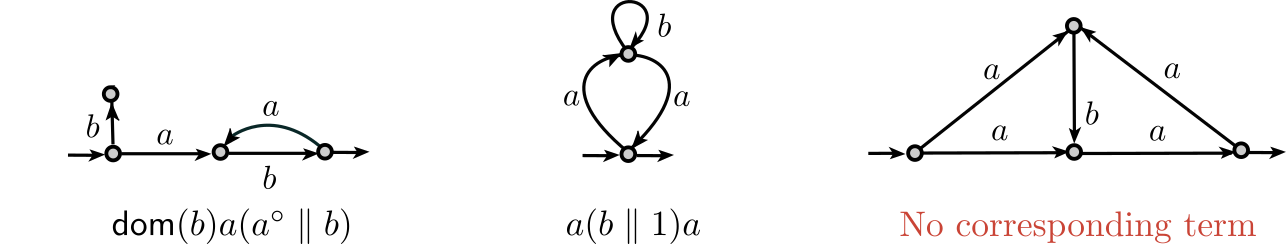
\includegraphics[scale=.35]{Pictures/example-graph}
 \end{center}
 \end{example}


  
\begin{definition}[$\TWT$ graphs]\label{def:graph-terms}
Consider the  signature $\sigma$ containing the binary operations $\cdot$ and $\parallel$, the unary operations ${\ }^\circ$ and $\dom$, and the nullary operations $1$ and $\top$. We define \emph{$\TWT$ terms} as the terms generated by the signature $\sigma$ and the alphabet $\Sigma$: 
\begin{align*}
t,u:=\  a\ \mid\ t\comp u\ \mid\ (t\parallel u)\ \mid \ t^\circ\ \mid\ \dom(t)\ \mid\ 1\ \mid \ \top \qquad \qquad a\in \Sigma
\end{align*}
We define the graph of a term $t$, $\G(t)$, by induction on $t$, by letting:  $$\begin{array}{l}
    
      \Gr 1=
               \begin{tikzpicture}[baseline=(0.south),xscale=.7]
                 \position (0) (0,0);
                           \initst (0); \fnst (0);
               \end{tikzpicture} \qquad
               \quad
                \Gr \top= 
               \begin{tikzpicture}[baseline=(0.south),xscale=.7]
                 \position (0) (0,0);
                 \position (1) (1,0);
                 \initst (0); \fnst (1);
               \end{tikzpicture}
           \qquad  \quad 
                \Gr a =  
              
\includegraphics[scale=1]{Pictures/unary-letter}
               \qquad
                  \quad         
                \Gr b= 
               \begin{tikzpicture}[baseline=(0.south),xscale=.7]
                 \position (0) (0,0);
                 \position (1) (1,0);
                 \initst (0); \fnst (1);
                 \edge[above] (0)(1)[b];
               \end{tikzpicture}
               \end{array} 
$$
and interpreting the operations of the syntax as follows:
$$\begin{array}{llllll}
 G\comp H&= &  \begin{tikzpicture}[baseline=(0.south),xscale=.7]
                  \position (0) (0,0);
                  \position (1) (1.5,0);
                  \position (2) (3,0);
                  \initst (0); \fnst (2);
                  \draw[arc] (0) 
                  to node[midway,fill=white,inner sep = 0] {$G$} (1);
                  \draw[arc] (1)
                  to node[midway,fill=white,inner sep = 0] {$H$} (2);
                \end{tikzpicture} 
                &\qquad\quad G\parll  H & =  & \begin{tikzpicture}[baseline=(0.south),xscale=.7]
                 \position (0) (0,0);
                 \position (1) (1.5,0);
                 \initst (0); \fnst (1);
                 \draw[arc] (0) to[bend left] 
                 node[midway,fill=white,inner sep = 0] {$G$} (1);
                 \draw[arc] (0) to[bend right]
                 node[midway,fill=white,inner sep = 0] {$H$} (1);
               \end{tikzpicture} \\[4pt]
               \dom(G)&= &
             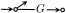
\includegraphics[scale=1]{Pictures/dom}  & \qquad\quad
                   G^\circ &= &
               \begin{tikzpicture}[baseline=(0.south),xscale=.7]
                 \position (0) (0,0);
                 \position (1) (1.5,0);
                 \initst (0); \fnst (1);
                 \draw[arc] (1)  
                 to node[midway,fill=white,inner sep = 0] {$G$} (0);
               
               \end{tikzpicture}  
  
\end{array} 
$$
In the picture above, we represent the graph $G$ by an arrow from its input to its output. For example, the graph $\dom(G)$ is obtained from $G$ by relocating the output to the input.  We usually write $tu$ instead of $t\comp u$ and give priorities to the symbols of $\sigma$ so that $ab\parll c$ parses to $(a\comp b)\parll c$.
We define the set of \emph{$\TWT$ graphs} as the graphs of the terms above. The graphs of $a$ and $a\parallel 1$, where $a\in \Sigma$, are called \emph{atomic}.
\end{definition}
We will sometimes identify terms with the graphs they generate. For example we may say that $(a\parallel b)$ is binary or connected to say that its graph is so.  

\begin{example} Below, from left to right, two $\TWT$ graphs and a graph which is not $\TWT$. 
\begin{center}
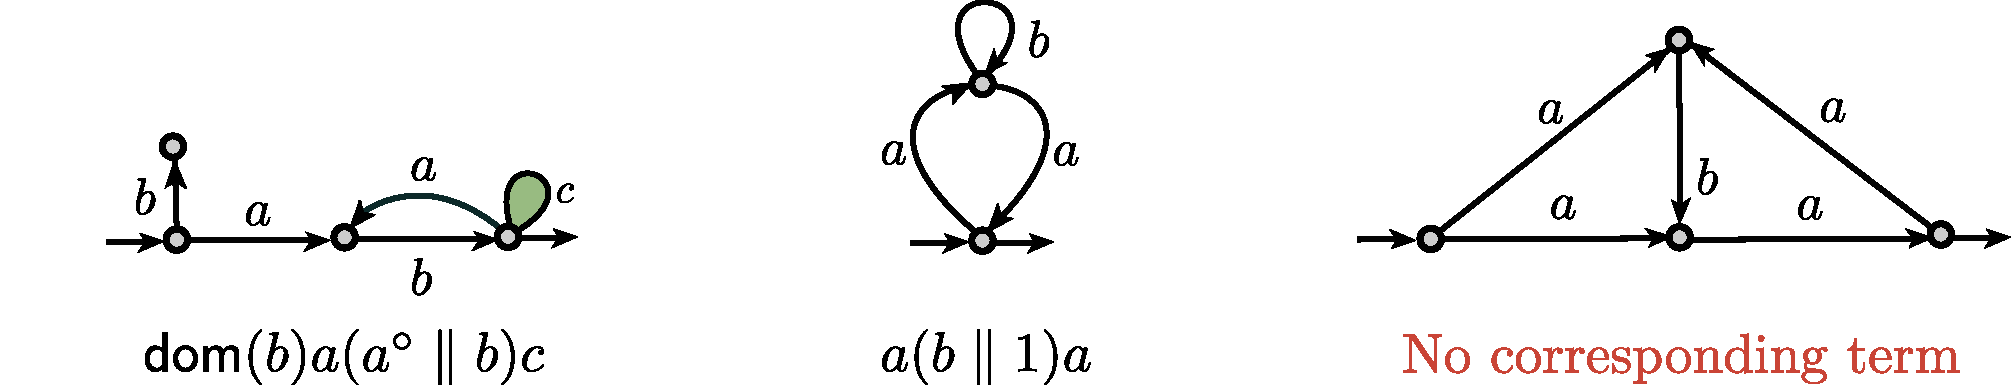
\includegraphics[scale=.35]{Pictures/example-graph-term}
\end{center}
\end{example}
%\begin{figure}
%
%\caption{Graph operations. \label{fig:graph-op}}
%\end{figure}
\begin{remark}
 The $\TWT$ graphs are exactly those graphs whose skeleton\footnote{The skeleton of a graph is the graph obtained by forgetting the labels and the orientation of the edges, and by adding an edge between the input and the output.} has tree-width 2~\cite{Cosme-LlopezP17}. 
\end{remark}

\begin{definition}[Graph languages]
Sets of graphs are called \emph{graph languages}.  A graph language is \emph{unary} or binary if all its graphs have this arity.
\end{definition}


\subsection{Counting monadic second-order logic}

We introduce $\CMSO$, the \emph{counting monadic second-order logic}, which is used to describe graph languages. 

\begin{definition}[The logic $\CMSO$]
Let $\mathcal{V}$ be the relational signature  which contains two binary symbols $\mathsf{source}$ and $\mathsf{target}$,   two unary symbols $\mathsf{input}$ and $\mathsf{output}$ and a unary symbol $a$ for each (unary or binary) letter $a\in \Sigma$. %We call the signature $\mathcal{V}$ the \emph{graphs vocabulary}.
\smallskip

Let $\mathbb{X}_1$ be a countable set of \emph{first-order variables} and $\mathbb{X}_2$  a countable set of \emph{set variables}
 The formulas of $\CMSO$  are defined as follows:
$$ \phi, \psi:= \  r(x_1,\dots, x_n) \ \mid \ x\in X \ \mid\ x=y \ \mid \ \exists x. \phi \ \mid \ \exists X. \phi \ \mid\ \phi\vee \psi\ \mid \ \neg \phi\ \mid \ \left(|X|\equiv k\right)\ [m]$$ 
 where $r$ is an n-ary symbol of $\mathcal{V}$,  $x_1,\dots,x_n, x\in \mathbb{X}_1$,  $X\in\mathbb{X}_2$ and $k,m\in\mathbb{N}$. \emph{Free and bound variables} are defined as usual. A \emph{sentence} is a formula without free variables. We use the usual syntactic sugar, for example $\phi\Rightarrow\psi$ as a shortcut for $\neg \phi\vee \psi$.
\end{definition}


We define the semantics of $\CMSO$ formulas. To handle free variables, $\CMSO$ formulas are interpreted over \emph{pointed graphs}.

\begin{definition}[Semantics of $\CMSO$] Let $G$ be a graph and $\Gamma$ be a set of variables. An \emph{interpretation} of $\Gamma$ in $G$ is a function mapping each first-order variable of $\Gamma$ to an edge or vertex of $G$, and each set variables to a a set of edges and vertices of $G$. A \emph{pointed graph} is a pair  $\langle G,I\rangle$ where $G$ is a graph and $I$ is an interpretation of a set of variables $\Gamma$ in $G$. If $\Gamma$ is empty, we denote it simply as $G$.   Let $\phi$ be a $\CMSO$ formula whose free variables are $\Gamma$ and let $\langle G,I\rangle$ be a pointed graph such that $I$ is an interpretation of $\Gamma$.  We define the \emph{satisfiability relation} $\langle G, I\rangle\models \phi$ as usual, by induction on the formula $\phi$. Here is an example of the semantics of some $\CMSO$ formulas:
\medskip

\noindent \begin{tabular}{rlrl}
$\mathsf{source}(v,e)$ :& the source of the edge $e$ is the vertex $v$.\quad\qquad & $\mathsf{input}(v)$ : & $v$ is the input of $G$.\\
$\mathsf{target}(e,v)$ :& the target of the edge $e$ is the vertex $v$. &
$\mathsf{output}(v)$ : & $v$ is the output of $G$.\\
$(|X|=k)[m]$ :& the size of $X$ is congruent to $k$ modulo $m$.& $a(e)$ :  &  $e$ is an $a$-edge.  \\[7pt]
\end{tabular}
If $\phi$ is a sentence, we define $\cL(\phi)$, the \emph{graph language of $\phi$} as  follows:
$$\cL(\phi)=\set{G \ \mid\ G \text{ is a graph and } G\models\phi}.$$
\end{definition}

\begin{definition}[$\CMSO$ definability]\label{def:CMSO-def}
A graph language is \emph{$\CMSO$ definable} if it is the graph language of  a $\CMSO$ sentence. 
\end{definition}

\begin{example} \label{ex:mso-def}The language of graphs having an $a$-edge
from the input to the output is definable in $\CMSO$, by the following formula for instance:
\begin{align*}
\phi:=\ \exists e.\ \exists i.\ \exists o.\ \mathsf{input}(i) \wedge \mathsf{output}(o)
\wedge a(e) \wedge \mathsf{source}(i, e) \wedge \mathsf{target}(e, o)
\end{align*}
Note that the graphs of this language may not be $\TWT$ graphs. 
\end{example}

\begin{example}
 The set of $\TWT$ graphs is a $\CMSO$ definable language. Indeed, $\TWT$ graphs are those graphs which exclude $K_4$, the complete graph with four vertices, as  minor. The set of graphs which exclude a fixed set of minors can be easily defined in $\CMSO$~\cite{Courcelle2012GraphSA}. 
 
 The set of $\TWT$ graphs having an $a$-edge from the input to the output is  definable in $\CMSO$, by the conjunction of the formula $\phi$ of Ex.~\ref{ex:mso-def} and the formula defining $\TWT$ graphs. 
  \end{example}

We state below a \emph{localization result}, which allows us to transform a $\CMSO$ sentence into another one which talks only about a part of the original graph. 

%To state it, we need the following notation: let $G$ be a graph, $s$ and $t$ be vertices of $G$ and $H$ be a set of edges and vertices. We write $(s,H,t)$ for the graph whose input and output are $s$ and $t$ respectively, whose sets of vertices and edges is the set of vertices and edges appearing in $H$, and which inherits the labeling function, the source and the target functions from $G$.

\begin{proposition}\label{prop:localization}
Let $\phi$ be a $\CMSO$ sentence, $x,y\in \mathbb{X}_1$ and $X\in\mathbb{X}_2$. There is a $\CMSO$ formula $\phi_{|(x,X,y)}$ such that, for every graph $G$ and  interpretation $I:(x\mapsto s, X\mapsto H, y\mapsto t)$, such that $(s,H,t)$ is a subgraph of $G$, we have:
$$ \langle G, I\rangle \models \phi|_{(x,X,y)}\qquad \Leftrightarrow \qquad (s, H, t) \models \phi$$
\end{proposition}

\begin{proof}
We construct $\phi|_{(x,X,y)}$ from $\phi$ as follows. First, we rename the variables of $\phi$ so that they become distinct from $x,y$ and $X$. Then we replace every subformula $\exists z.\ \psi$ by $\exists z.\ (z\in X)\wedge \phi$, every subformula $\exists Z.\ \psi$ by $\exists Z.\ (Z\subseteq X)\wedge \phi$,  every formula $\mathsf{input}(z)$ by $(z=x)$ and every formula $\mathsf{output}(z)$ by $(z=y)$.
We show that $\phi|_{(x,X,y)}$ has the intended semantics by induction on $\phi$. 
\end{proof}

\begin{remark} There is another  presentation of the syntax of $\CMSO$, where we remove first-order variables and the formulas including them, and  add the following formulas:
$$ X\subseteq Y\ \text{ and } \ r(X_1\dots, X_n) \quad \text{where $r$ is an $n$-ary symbol of $\mathcal{V}$.}$$
The formula $X\subseteq Y$ is interpreted as ``$X$ is a subset of $Y$'' and $r(X_1\dots, X_n)$ as ``for each $i$, $X_i$ is a singleton containing $x_i$ and $r(x_1\dots, x_n)$''.  This presentation is more convenient in proofs by induction as there are less cases to analyze. 
\end{remark}


\subsection{Recognizability}
 We can specify languages of graphs by means of $\sigma$-algebras, generalizing to graphs the notion of recognizability by monoids.  A \emph{$\sigma$-algebra} $\A$ is the collection of a set $D$ called its \emph{domain}, and for each $n$-ary operation  $o$ of $\sigma$, a function $o^\A:D^n\to D$.
 A homomorphism $h:\A\to \B$ between two $\sigma$-algebras $\A$ and $\B$ is a function from the domain of $\A$ to the domain of $\B$  which preserves the operations of $\sigma$.  Note that the set of $\TWT$ graphs, where the operations of $\sigma$ are interpreted as in Def.~\ref{def:graph-terms}, forms a $\sigma$-algebra which we denote by $\G_\TWT$.
  

\begin{definition}[Recognizability]
 We say that a language $L$ of $\TWT$ graphs is \emph{recognizable} if there is a $\sigma$-algebra $\A$ with finite domain, a homomorphism $h:\G_\TWT\to \A$ and a subset $P$ of the domain of $\A$ such that $L=h^{-1}(P)$.
\end{definition}

\begin{theorem}\label{thm:CMSO->Rec}
If a language of $\TWT$ graphs is $\CMSO$ definable, then it is recognizable.
\end{theorem}

\begin{proof} 
This result is proved in a more general framework in \cite{Mikolaj-long}. To adapt this to our setting, we just have to verify that our $\sigma$-algebras are also compatible with product and powerset operations. This is straightforward, as our algebras are very similar to those in \cite{Mikolaj-long}.
\end{proof}

\subsection{Operations on graph languages}\label{sec:op-lang}

The operations of $\sigma$ can be lifted from graphs to graph languages in the natural way. We say that an operation on graph languages is \emph{$\CMSO$ compatible} if, whenever its arguments are $\CMSO$ definable, then so is its result. 

%For example if $L$ and $M$ are graph languages, we can define $L\comp M$ as follows:
%$$ L\comp M=\set{G\comp H\ \mid \ G\in L \text{ and } H\in M}$$
%We usually write $L M$ instead of $L\comp M$.
\begin{proposition}\label{prop:CMSO-def-operations}
Union and the operations of $\sigma$ are $\CMSO$ compatible.
\end{proposition}
\begin{proof}
The language of $\phi  \vee \psi$ is the union of the languages of $\phi$ and $\psi$, for every $\CMSO$ sentences $\phi$ and $\psi$, this concludes the case of union.

For the operations of $\sigma$, we use the localization result. We treat the case of series composition, the other operations can be treated similarly. Let $\phi$ and $\psi$ be two $\CMSO$ sentences. We construct the formula $\phi\cdot\psi$ as follows. We guess two sets $X$ and $Y$ and an element $m$, which are intended to be the graph coming from $\phi$, the graph coming from $\psi$ and the middle vertex in between them, respectively. Then we say that $X$ contains the input, $Y$ contains the output and that $X$ and $Y$ intersect exactly in $m$. Using the localization result, we say that the graph whose set of edges and vertices is $X$,  whose input is the input of the original graph, and whose output is $m$ satisfies $\phi$. We say similarly that  the graph whose set of edges and vertices is $Y$, whose input is $m$ and whose output is the output of the original graph satisfies $\psi$.
\begin{align*}
\phi\cdot\psi:= \ \exists X,\ \exists Y,\ \exists m,\ \exists i,\ \exists  o.\ \ &\mathsf{input}(i)\wedge \mathsf{output}(o)\wedge (i\in X) \wedge (o\in Y) \wedge (X\cap Y=\set{m}) \\ & \wedge \phi|_{i,X, m} \wedge \psi|_{m,Y,o}
\end{align*}
where $(X\cap Y=\set{m})$ is a $\CMSO$ formula saying that the intersection of $X$ and $Y$ is  $m$. 
 \end{proof}

 We define two additional operations: \emph{substitution} and \emph{iteration}.
 
 \begin{definition}[Substitution and iteration]
  Let $x$ be a letter, $L$ and $M$ be $\TWT$ graph languages and let be $G$ a $\TWT$ graph. We define the set of graphs $G[L/x]$ by induction on $G$ as follows:
\begin{align*}
x[L/x]=L, \quad a[L/x]=a\ (a\neq x)\quad\text{and}\quad o(G_1\dots, G_n)[L/x]=o(G_1[L/x],\dots,G_n[L/x])  
\end{align*}
where $o$ is an $n$-ary operation of $\sigma$. We define $M[L/x]$ as:
$$ M[L/x]=\underset{G\in M}{\bigcup} G[L/x]$$
We define similarly the simultaneous  substitution $M[\vec{L}/\vec{x}]$, where $\vec{L}$ and $\vec{x}$ are  respectively a list of $\TWT$ graph languages and a list of letters of the same length.  
\smallskip

For every $n\geq 1$, we define the language $L^{n,x}$ and the iteration $\mu x. L$ as follows:
\begin{align*}
\qquad \qquad L^{1,x}:=L,\qquad L^{n+1,x}=:L[L^{n,x}/x]\cup L^{n,x}, \qquad \mu x. L:= \underset{n\geq 1}{\bigcup} L^{n,x}.
\end{align*}
\end{definition}


\begin{remark}
Substitution and iteration are not $\CMSO$ compatible in general. For instance, the iteration of the $\CMSO$ language $\set{axb}$, which is the set  $\set{a^nxb^n \mid n\in \mathbb{N}}$, is not $\CMSO$ definable.  
However, under a \emph{guard condition} that we introduce later, we recover $\CMSO$ compatibility.
\end{remark}

We finally consider two restricted forms of iteration called \emph{Kleene} and  \emph{parallel iteration}.

%Let $L$ be a graph language and $x$ a letter with the same arity as $L$. 
\begin{definition}[Kleene and parallel iteration]
We define the \emph{Kleene iteration} $L^+$ and the \emph{parallel iteration} $L^\parallel$ of a language $L$ as follows, where $x$ is a letter not appearing in $L$:
\begin{align*}
\qquad \qquad \quad \quad L^+=(\mu x.\ L\comp x)[L/x],\qquad \qquad L^{\parll} =(\mu x.\ L
\parll  x)[L/x].
\end{align*} 
\end{definition}


%\subsection{The structure of $\TWT$-graphs}
%This section can be skipped at first, it will not be used until Sec.~\ref{}.
%
%
%\begin{definition}[Series and parallel decompositions]
%Let $G$ be a $\TWT$-graph.
%
%\noindent A \emph{list decomposition} of $G$ is a list $S$ of $\TWT$-graphs  such that $G$ is isomorphic the series composition  of the elements of $S$, respecting the order of $S$.  
%
%\noindent A \emph{multiset decomposition} of $G$ is a triplet $(L, P, R)$ of multisets of $\TWT$-graphs satisfying:
%$$G=\parll  L\ \cdot\parll  P\ \cdot \parll  R$$
%A  series (resp. parallel) decomposition of $G$ is the set of all $\TWT$-graphs appearing in some list (resp. multiset) decomposition, distinct from $1$ and $\top$.   
%A series (resp. parallel) decomposition of $G$ is \emph{trivial} if it is equal to $\set{G}$.
%\end{definition}
%\begin{example}
%\end{example}
%\begin{proposition}
%Let $G$ be a connected $\TWT$-graph. 
%Maximal series (resp. parallel) decompositions of $G$ are unique. We denote them $\mathsf{msd}(G)$ and  $\mathsf{mpd}(G)$ respectively. 
%\end{proposition}
%
%\begin{definition}[Pure graphs]
%A $2$p-graph is \emph{atomic} if it is the graph of a letter or a term $a\parll  1$, where $a\in A$. A $2$p-graph $G$ is \emph{pure} if it is connected, not atomic, and its series or parallel decomposition is trivial. When $G$ is pure, we distinguish 3 cases:
%\begin{itemize}
%\item $G$ is binary and $\mathsf{mpd}(G)$ is trivial. In this case we write $G:\mathsf{s}$.
%\item $G$ is binary and $\mathsf{msd}(G)$ is trivial. In this case we write $G:\mathsf{p}$.
%\item $G$ is unary and $\mathsf{mpd}(G)$ is trivial.  We write $G:\mathsf{d}$.
%\end{itemize} 
%\end{definition}
%In this case, we have also that $\mathsf{mpd}(G)$ is trivial.
%\begin{example}
%\end{example}
%
\subsection{Pure graphs and modules}

\begin{definition}[Pure graphs.]
Let $G$ be a graph. If we remove the interface vertices of $G$ we obtain one or several connected components which we call the \emph{faces} of $G$. 
The \emph{arity of a face} is the number of interface vertices of $G$ it is incident to. 
\begin{center}
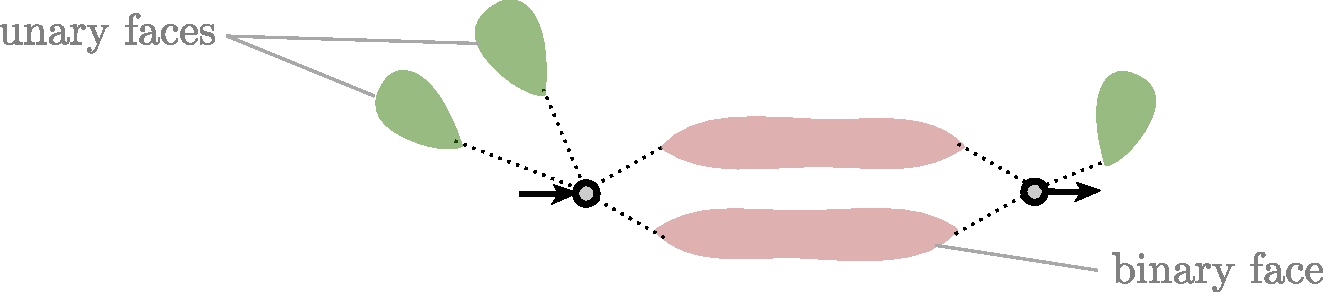
\includegraphics[scale=.4]{Pictures/unary-and-binary-faces}
\end{center}
\noindent We say that $G$ is \emph{pure} if  it has at least one face and  all it faces have the same arity as itself.  We say that $G$ is \emph{prime} if it has exactly one face, and \emph{composite} if it has at least two faces. 
\end{definition}


   \begin{remark} Pure graphs are connected and non-empty.  Not all graphs are pure.
   \end{remark}

   \begin{definition}[Type of a pure graph]
The \emph{type} of a pure graph is a pair specifying its arity and whether it is prime or composite. We say that a graph is \emph{series} if it is binary and prime, \emph{parallel} if it is binary and composite, \emph{domain} if it is unary and prime and \emph{test} if it is unary and composite. We denote by $\mathsf{s}, \mathsf{p}, \mathsf{d}$ and $\mathsf{t}$ the type series, parallel, domain and test respectively. Series, parallel domain and test graphs look like this:
   \begin{center}
   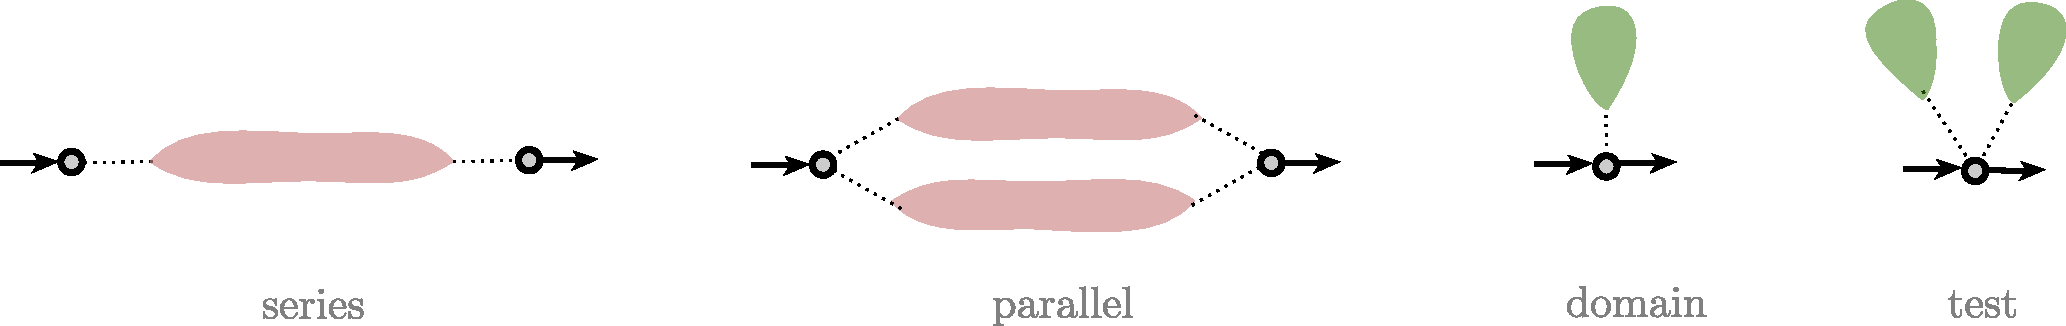
\includegraphics[scale=.4]{Pictures/spdt}
   \end{center}
   A graph language is (of type) \emph{series}, \emph{parallel}, \emph{domain} or \emph{test} if \textbf{all} its graphs have this type.  
   \end{definition}
   
   There is a canonical way to decompose pure graphs of type series, parallel and test. 
 \begin{proposition}[\cite{Damien}]
 Let $G$ be a pure graph. The graph $G$ has the following shape:
 $$\begin{array}{llll}
 G&:=&  P_0\cdot U_1 \cdot P_1 \dots U_n\cdot P_n & \qquad \qquad\text{ if $G$ is series,}\\[3pt]
 G&:=&  \ S_0\parallel  \dots \parallel S_n &  \qquad \qquad\text{ if $G$ is parallel,}\\[3pt]
 G&:=&  D_0\parallel  \dots \parallel D_n &  \qquad \qquad\text{ if $G$ is test,}\\
 \end{array}$$
 $P_j$ being parallel or atomic, $U_i$ unary, $S_i$ series and $D_i$ domain, for all $j\in[0,n], i\in[1,n]$.
\end{proposition}
Here is a picture illustrating this proposition:
\begin{center}
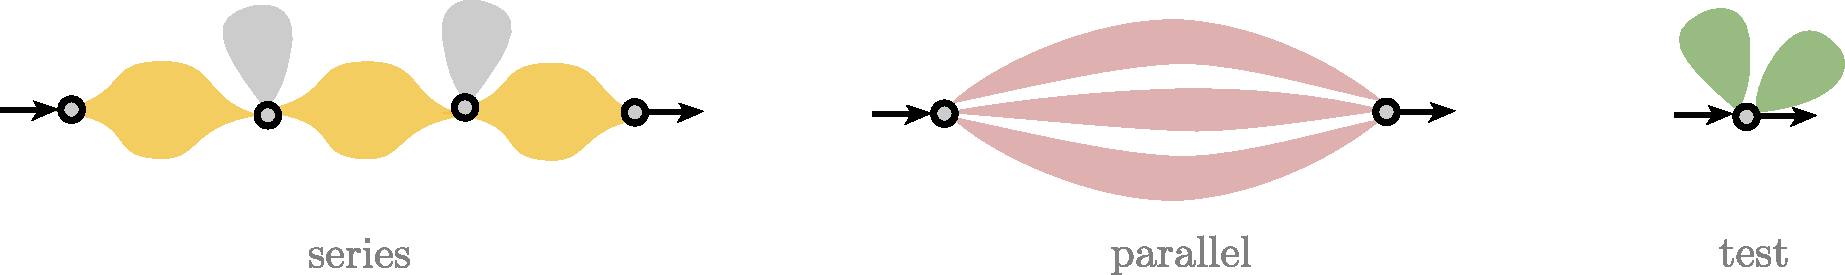
\includegraphics[scale=.35]{Pictures/spt}
\end{center}
\begin{definition}[Contexts]
%A \emph{context} is a graph with a unique edge, labeled by a special letter, called its \emph{hole}.  If $C$ is a context whose hole is $h$ and $H$ a graph \textbf{with the same arity as $h$}, we define $C[H]$ as the graph obtained from the disjoint union of $C$ and $H$, by removing the edge $h$,  identifying the input of $h$ with the input of $H$, the output of $h$ with the output of $H$, and  by letting the interface of $C[H]$ to be that of $C$. 
Let $\mathbb{S}$ be a set of \emph{special (unary and binary) letters}, and let $n\geq 1$. An \emph{$n$-context}  is a graph such that $n$ of its edges, called \emph{holes}, are numbered from $1$ to $n$, and labeled by $n$ distinct special letters.  We call $1$-contexts simply \emph{contexts}.

Let $C$ be an $n$-context whose holes are $h_1\dots,h_n$ and let $H_1,\dots,H_n$ be graphs such that $h_i$ and the $H_i$ have the same arity, for all $i\in [1, n]$.  We define $C[H_1,\dots,H_n]$ as the graph obtained from the disjoint union of $C$ and $H_1,\dots, H_n$, by removing the holes of $G$, and for every $i\in[1,n]$  identifying the input of $h_i$ with the input of $H_i$, the output of $h_i$ with the output of $H_i$, and  by letting its interface of  to be that of $C$.
\end{definition}

\begin{definition}[Islands and modules]  
An \emph{island} of a graph $G$ is a graph $H$ such that there is a context $C$ satisfying $G=C[H]$.  A \emph{module} is a island which is pure.  Two islands (or modules) of a graph are \emph{parallel} if they have the same interface. 

\noindent Since modules are pure, we can speak of series, parallel, domain and test modules  of a graph. 
\end{definition}

The following picture illustrates a unary and binary island of a graph.
\begin{center}
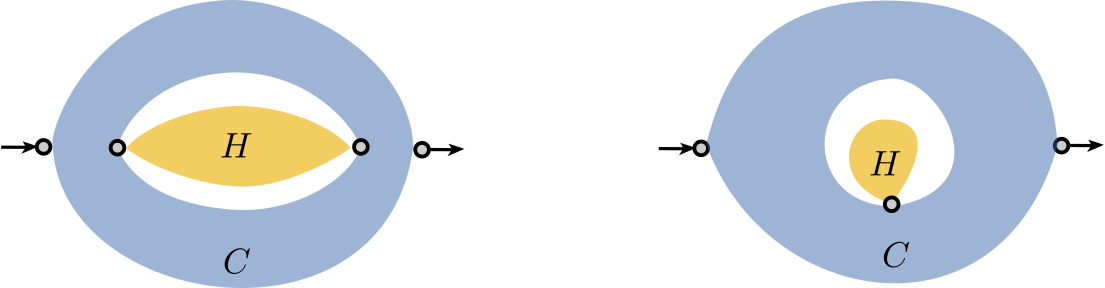
\includegraphics[scale=.35]{Pictures/island}
\end{center}
\begin{remark} Our notion of modules is different from the one usually used in graph theory, more precisely in the setting of \emph{modular decompositions}. %There, $X$ is a module if, for each vertex $v \not\in X$, either every member of $X$ is a non-neighbor of $v$ or every member of $X$ is a neighbor of $v$.
\end{remark}
 
 \begin{remark}
If $I$ is an interface in a graph $G$,  there is always an island of $G$ whose interface is $I$, the empty graph for example. This is not the case for modules.   
\end{remark}

\begin{remark}
The parallel composition of two islands of a graph $G$ with the same interface is also an island of $G$ with the same interface. Similarly, the parallel composition of two modules of a graph $G$ with the same interface is also a module of $G$ with the same interface. This justifies the following definition.
\end{remark}

\begin{definition}[Maximal islands and modules]
 Let $G$ be a graph and $I$ an interface in $G$.  The \emph{maximal island  at $I$} is the parallel composition of all the islands of $G$ whose interface is $I$, we denote it by $\mathsf{max}\text{-}\mathsf{island}_G(I)$. The \emph{maximal module at $I$} is the parallel composition of all the modules of $G$ whose interface is $I$, we denote it by $\mathsf{max}\text{-}\mathsf{module}_G(I)$.
\end{definition}
\begin{remark}
The maximal module at a given interface does not always exist.
\end{remark}

\begin{proposition}\label{prop:pure-modules-are-CMSO}
Being series, parallel, domain, test, an island, a module, a maximal island, a maximal module are $\CMSO$ definable properties. 
\end{proposition}
\begin{proof} We propose an equivalent definition for islands which is more convenient to express in $\CMSO$.
\begin{lemma}\label{lem:module} Let $G$ be a graph. A  subgraph $H$ of $G$ is an island iff no interface vertex of $G$ in an inner vertex of $H$ and there is no edge from an inner vertex of $H$ to a vertex of $G$ outside of $H$.
\end{lemma}
\begin{proof}
It is easy to see that if $H$ is an island, then it satisfies  these conditions.
Suppose that $H$ satisfies the conditions of the lemma. Let $C$ be the graph obtained from $G$ by removing all the edges and the inner vertices of $H$ and by adding a edge labeled by a special letter, with the same interface as $H$. It is easy to see that $C[H]$ is $G$.
\end{proof}
In $\CMSO$, we can express that a graph is not a maximal module: there is a module with the same interface, which is strictly bigger. Hence we can express maximality.

Since connectivity is expressible in $\CMSO$, we can express easily in $\CMSO$ that a subgraph is a face. We can also say if a a graph is series, by saying that it has a unique face, and this face is binary. We can proceed similarly to express that a graph is parallel,  domain, test and pure. Finally, we express that a graph is a module by saying that it is an island which is pure.    
\end{proof}


\section{Regular expressions for $\TWT$ graphs}\label{sec:reg-exp}


\subsection{Regular expressions for word and multiset graphs}
\begin{definition}[Word and multiset alphabets]
Let $\Sigma_\mathsf{w}$ be the set of terms whose graphs have the following form, where $a,b\in \Sigma_2$ and $c\in \Sigma_1$:
\begin{center}
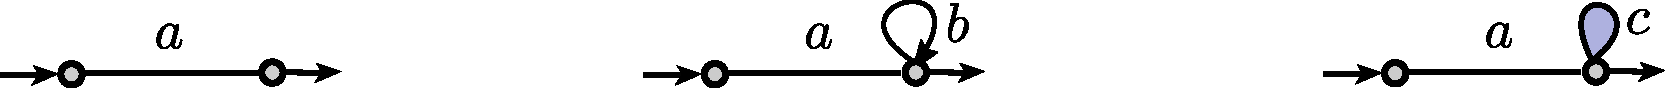
\includegraphics[scale=.37]{Pictures/word-alphabet}
\end{center}
Let $\Sigma_\mathsf{m}$ be the set of terms whose graphs have the following form, where $a\in \Sigma_2$ and $b\in \Sigma_1$:
\begin{center}
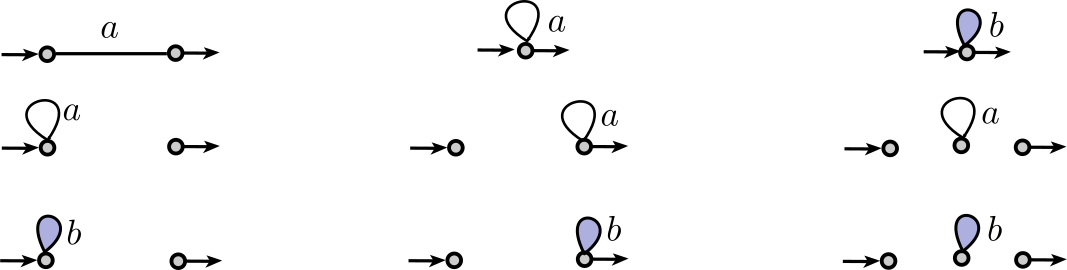
\includegraphics[scale=.35]{Pictures/multiset-alphabet}
\end{center}
 \emph{Word graphs} are the graphs generated from those of $\Sigma_\mathsf{w}$ by series composition,  and \emph{multiset graphs} are the graphs generated from those of $\Sigma_\mathsf{m}$ by parallel composition. 
\end{definition} 
\begin{example}
Below, from left to right, a word graph and two multiset graphs.
\begin{center}
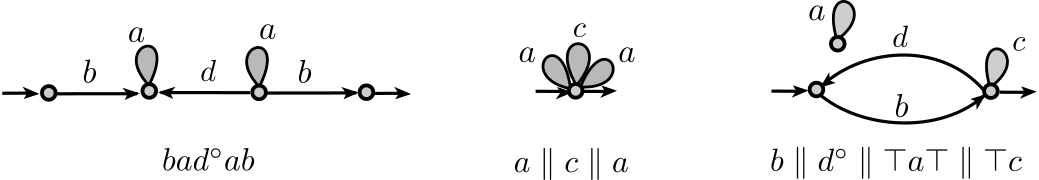
\includegraphics[scale=.4]{Pictures/word-and-multiset-graphs}
\end{center}
\end{example}
\begin{definition}[Word an multiset expressions]
\emph{Word expressions} are defined as follows:
\begin{align*}
\qquad\qquad \qquad e,f := a\ \mid \ e\cdot f\ \mid \ e\cup f\ \mid \ e^+\qquad (a\in \Sigma_\mathsf{w})
\end{align*}
\emph{Multiset pre-expressions} are defined  as follows:
\begin{align*}
\qquad\qquad \qquad e,f := a\ \mid \ (e\parallel f) \ \mid \ e\cup f\ \mid \  e^\parallel\ \qquad (a\in \Sigma_\mathsf{m})
\end{align*}

\emph{Multiset expressions} are those pre-expressions, where each sub-term appearing under a parallel iteration, is built using a  single element $a\in \Sigma_\mathsf{m}$ (all the other operations are allowed). The graph language of an expressions is defined as usual. 
\end{definition}
%We say that a graph language is \emph{word-regular}  or \emph{multiset-regular} if it is the language of a word or a  multiset  regular expression.
\begin{remark}
To see why the condition on multiset regular expressions is useful, consider the expression $e=(a\parll b)$. The language of its parallel iteration is the set of multiset graphs which have the same number of $a$-edges and $b$-edges, and this is  not  a $\CMSO$ definable language. 
\end{remark}


\subsection{Context-free expressions}

\begin{definition}[Context-free expressions]
We define \emph{context-free expressions} as the set of terms generated by the following syntax:
\begin{align*}
\qquad\qquad \qquad e,f := &\ \ \ e_\mathsf{w}\ \mid\ e_\mathsf{m}\\
       & |\ e\cdot f \ \mid\ \  (e \parallel f)\ \ \mid\ \ e^\circ  \ \ \mid\ \dom(e) \ \mid\ 1\ \mid\ \top \\
       & |\ e\cup f \ \mid\  e[f/x] \ \mid\ \mu x. e
\end{align*}
where $e_{\mathsf{w}}$ and $e_{\mathsf{m}}$ are respectively word and multiset regular expressions.  We define the \emph{language} of a context-free expression $e$, denoted $\cL(e)$, by induction on $e$, interpreting the operations of the syntax as described in Sec.~\ref{sec:op-lang}. 
\end{definition}
\emph{Regular expressions for $\TWT$ graphs} will be defined as a restriction of context-free expressions, where substitution and iteration are allowed only under a \emph{guard condition} that we shall explain in the following. 
 



\subsection{The guard condition}

\begin{definition}[Guarded letters]
Let $G$ be a graph and $x$ a letter. We say that:
\begin{itemize}
\item $x$ is \emph{$\mathsf{s}$-guarded in $G$} if $x$ is binary and every $x$-labeled edge of $G$ is parallel to a module.
\item $x$ is \emph{$\mathsf{p}$-guarded in $G$} if $x$ is binary and no $x$-labeled edge of $G$ is parallel to a module.
\item $x$ is $\mathsf{d}$-guarded in $G$ if $x$ is unary.
\item $x$ is $\mathsf{t}$-guarded in $G$ if $x$ is unary and no $x$-labeled edge of $G$ is parallel to a module.
\end{itemize} 
Let $\tau\in\set{\mathsf{s}, \mathsf{p}, \mathsf{d}, \mathsf{t}}$ be a type and $L$ a graph language. We say that \emph{$x$ is $\tau$-guarded} in $L$ if it is $\tau$-guarded in every graph of $L$.
\end{definition}
%\begin{example}
%\todo{add a picture?}
%\end{example}
\begin{definition}[Guard condition] Let $x$ be a letter, $M$ a $\TWT$ graph language and $L$ a pure language of type $\tau$.
The substitution $M[L/x]$ is guarded if $x$ is $\tau$-guarded in $M$.
The iteration $\mu x. L$ is guarded if $x$ is $\tau$-guarded in $L$.

We say that the iteration \emph{$\mu x. L$ is of type $\tau$} if $L$ is of type $\tau$.
\end{definition}


\begin{definition}[Regular expression]
A \emph{regular expression} is a context-free expression where every substitution and iteration is guarded. A language of graphs is \emph{regular} if it is the language of some regular expression. 
\end{definition}
\begin{remark}
When $L$ is test and $x$ is a unary letter, then $\mu x. L$ is always guarded. 
\end{remark}
 

%The following properties show that the guard condition behaves well with substitution and iteration, and that it is a decidable property among context-free expressions.
%
%\begin{proposition}\label{prop:guard-preservation} Let $L$ and $M$  be languages of $\TWT$ graphs. \todo{update}
%\begin{itemize}
%\item If $x$ is guarded in $L$, then $x$ is  guarded in $\mu x. L$.
%\item If $x$ is guarded in $L$ and $M$, then $x$ is guarded in $M[L/x]$.
%\end{itemize}
%\end{proposition}


\begin{proposition}\label{prop:decidability}
We can decide if a  context-free expression is regular.
\end{proposition}
\begin{proof}[Proof sketch]We can annotate our regular expressions with extra information, remembering whether their language is pure, unary, binary, and in
general what type of graphs it generates. This allows us to check the
guard condition and propagate the annotations inductively, using the
syntax tree of the expression.  We start from the leaves of this tree
(labeled by atomic formulas) and propagate the annotations upwards while
verifying the guard condition when required, until we reach the root of
the tree (labeled by the full expression).
\end{proof}
\begin{remark}
Be aware that prop.~\ref{prop:decidability} is about deciding a syntactic property of $e$, namely that the iterations and substitutions are guarded. However, the problem of determining if a context-free expression \emph{defines a $\CMSO$ language} is undecidable. This apparent contradiction comes from the fact that  some context-free expressions, which are not guarded, define $\CMSO$ languages, as we shall see in the upcoming examples.
\end{remark}



\subsection{Examples}



 


\begin{example} The iteration $\mu x. axb$ is not guarded. Indeed, the language of $axb$ is series, as it contains a single series graph $G$. However, the letter $x$ is not $\mathsf{s}$-guarded in $G$, because it is not parallel to any module of $G$. The graph of this iteration look like this:
\begin{center}
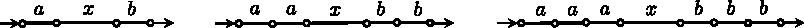
\includegraphics[scale=1]{Pictures/expl0.pdf}
\end{center}
\end{example}
 
 \begin{example} The iteration $\mu x. a(x\parallel c)b$ is guarded. Indeed the language of $a(x\parallel c)b$ is series, actually it contains a single graph $G$, depicted below left, which is series. The letter $x$ is $\mathsf{s}$-guarded in $G$, because it is parallel to a module, namely the $c$-edge.   The graph of this iteration look like this:
\begin{center}
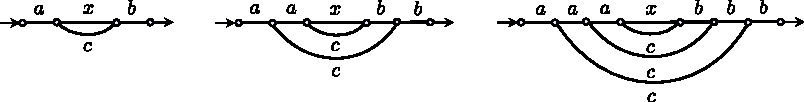
\includegraphics[scale=1]{Pictures/expl1.pdf}
\end{center}
%The language of this expression, while very similar to that of the previous example, is $\CMSO$ definable. 
\end{example}

%It might be surprising that this graph is r somehow the $c$-edges permettent de se repereer dans le graphe. 

Note the similarity between the graph language of $\mu x. axb$ and that of $\mu x. a(x\parallel c)b$: the former is obtained by forgetting the $c$-edges of the latter. Yet, the latter is $\CMSO$ definable, while the former is not. In the case of $\mu x. a(x\parallel c)b$, the $c$-edges will guide a $\CMSO$ formula to relate the $a$-edges and the $b$-edges of the same iteration depth.  This is the main intuition behind the guard condition for series languages.  
%\textcolor{red}{This is a good time to give the intuition on the guard condition.}
 \begin{example}
The iteration $\mu x. (axa\parallel axa)$ is guarded. Indeed, the language of $(axa\parallel axa)$ is parallel, as it contains a unique graph $G$ (the left graph below) which is parallel. The letter $x$ is $\mathsf{p}$-guarded because all the occurrences of $x$ are not parallel to any module of $G$.
Note that the graphs of this expression have the following shape: they all start with  a binary tree whose edges are labeled by $a$, end ends with the mirror image of this tree, while the corresponding leafs are connected by an $x$-edge.  Those trees are colored in red below. 
\begin{center}
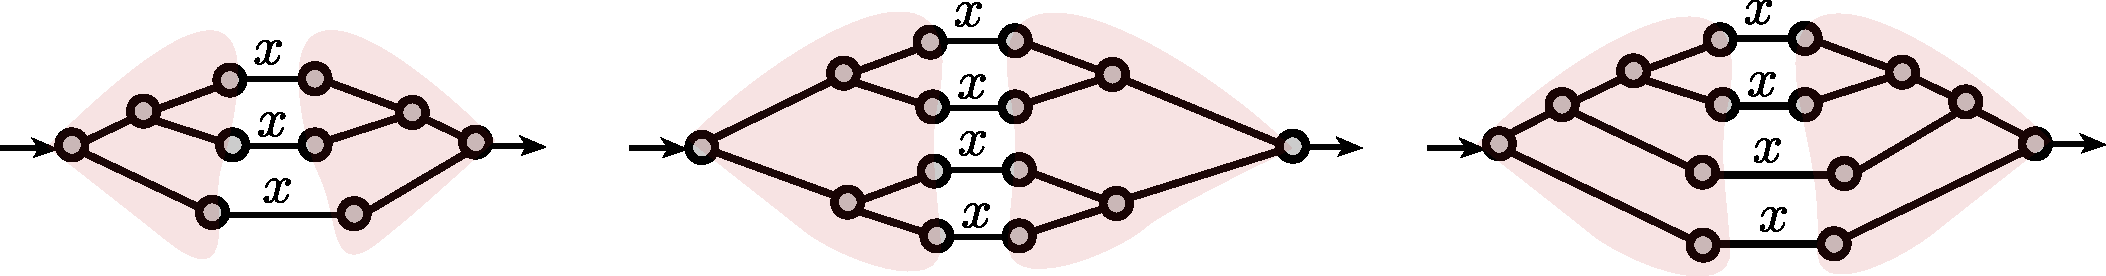
\includegraphics[scale=.35]{Pictures/TxT.pdf}
\end{center}
At first glance, this expression dos not seem to be $\CMSO$ definable, as it seems that we need to test whether a graph starts and ends with the same tree. We will see however that the language of this expression, as those of all regular expressions, is $\CMSO$ definable.  
\end{example}

The guard condition is not ``perfect'', in the sense that some non-guarded context-free expressions might  generate $\CMSO$ definable languages, as shown in   the following example.

\begin{example}
 The context-free expression $(\mu x. axb)[1/a, 1/x, 1/b]$ is not regular because the iteration $\mu x. axb$ is not guarded. However its language, the  graph of $1$,   is $\CMSO$ definable.
\end{example}

\begin{remark}
Intuitively, the guard condition allows only those graphs where series and parallel operations alternate. This why we add the word and multiset expressions: to allow graphs where we can iterate only series or parallel operations respectively.
\end{remark}

\subsection{Main result}

The main result of this paper is the following theorem:
\begin{theorem}
Let $L$ be a language of $\TWT$ graphs. We have:
$$L \text{ is recognizable}\qquad \Leftrightarrow \qquad L \text{ is $\CMSO$ definable}  \qquad \Leftrightarrow \qquad L \text{ is regular}$$
%$$\begin{tikzcd}
%               &  L \text{ is recognizable} \arrow[rd, Rightarrow, "(2)"] &  \\[-.5cm]
%L \text{ is $\CMSO$ definable}\arrow[ru, Rightarrow, "(1)"] & \qquad\qquad\qquad\qquad\qquad\qquad\qquad\qquad & L \text{ is regular} \arrow[ll, Rightarrow, "(3)"] 
%\end{tikzcd}$$
%\begin{center}
%$L$ is $\CMSO$-definable $\quad\Leftrightarrow\quad$ $L$ is recognizable $\quad\Leftrightarrow\quad$ $L$ is regular
%\end{center}
\end{theorem}
Thanks to Thm.~\ref{thm:CMSO->Rec}, $\CMSO$ definability implies recognizablity. We show that regularity implies $\CMSO$ definability in Sec.~\ref{sec:reg->def} and  that recognizabilty implies regularity in Sec.~\ref{sec:rec->reg}. 
\section{Companion relations}\label{sec:comp-rel}



 


\begin{definition}[Companion relation] Let $G$ be a graph. 
Two paths  of $G$ are \emph{orthogonal} if they do not share any edge, and whenever they share a vertex, it is necessarily an interface vertex of one of them. A set of paths is a \emph{set of orthogonal paths} if its paths are pairwise orthogonal.

A relation $R$ on the vertices of $G$ is a \emph{companion relation} if there is a set of orthogonal paths $P$ such that $(v,w)\in R$ iff $(v,w)$ is the interface of a path $p\in P$. We say that $p$ is a \emph{witness} for $(v,w)$, and that $P$ is a \emph{witness} for the relation $R$.
\end{definition}

\begin{example} \label{ex:guared-set-of-paths}
The relation indicated by the green dotted arrows below is a companion relation. This is not the case for the one indicated by the red dotted arrows.
\begin{center}
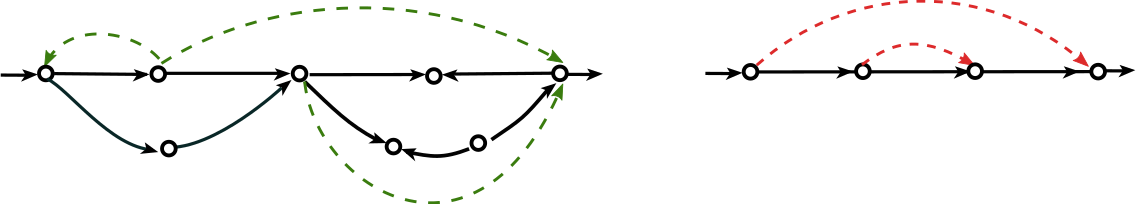
\includegraphics[scale=.4]{Pictures/guarded-set-of-paths}
\end{center}
 \end{example}

We introduce $\CMSO^r$, an extension of $\CMSO$ where quantification over companion relations is possible.

\begin{definition}[The logic $\CMSO^r$] 
  Let $\mathbb{X}_r$ be a set of \emph{relation variables}, whose elements are denoted $R, S, \dots$. The formulas of $\CMSO^r$ are of the following form:
\begin{align*}
 \phi :=&\ \CMSO\ |\ \exists R.\ \phi\ |\ (x,y)\in R & \qquad (R\in \mathbb{X}_r,\ x,y\in\mathbb{X}_1).
\end{align*}
\end{definition}
 
 As for $\CMSO$, we need to define the semantics of a formula over pointed graphs to handle free variables.
 
\begin{definition}[Semantics of $\CMSO^r$]
Let $G$ be a graph and $\Gamma$ be a set of variables.  An interpretation of $\Gamma$ is as usual, but here every relation variable is mapped to a binary relation on the vertices of $G$.  We define the \emph{satisfiability relation} $\langle G, I\rangle\models \phi$ as usual, by induction on the formula $\phi$. The only new cases are the quantification  $\exists R$ which is interpreted as ``there exists a companion relation $R$ on the vertices of the graph'', and the formulas $(x,y)\in R$ which are interpreted as ``there is a pair of vertices $(x,y)$ in $R$''. 
\end{definition}


\subsection{The logic $\CMSO^r$ have the same expressive power as $\CMSO$}
%A \emph{path} in a graph is a non-empty connected module, which becomes disconnected when we remove one of its edges. A \emph{directed path}, is path whose  vertices can be totally ordered (the input being the least element and the output the greatest element), such that each consecutive vertices are connected by an edge from the smallest to the biggest.



To guess a companion relation in $\CMSO$, we show how to encode a set of guarded paths by a collection of sets called a \emph{footprint}.


\begin{definition}[Frontier edges of a path] Let $p=(v_0,e_1,v_1,\dots,e_n,v_n)$ be a path. If $n>1$, we call $e_1$ the \emph{opening edge} of $p$ and $e_n$ its \emph{closing edge}. If $n=0$, we call $e_0$ its \emph{single edge}.  Opening, closing and single edges are called the \emph{frontier edges} of $p$, the other edges are called its \emph{inner edges}.  
 \end{definition}


 
 \begin{definition}[Footprint] A \emph{footprint} in a graph $G$  is the following collection of data: a partition of the vertices of $G$ into \emph{non-path} and \emph{path} vertices, a partition of edges into \emph{non-path} and \emph{path} edges, a partition of path edges into \emph{frontier} and \emph{inner} edges, a partition of frontier edges into \emph{opening, closing and single} edges and a partition of path edges into \emph{direct} and \emph{inverse} edges.
 
 The partition of path edges into direct and inverse ones provides them with a new orientation:  they conserve their original  orientation if they are direct, or get reversed (we swap the source and target) if they are inverse edges.  
 
 Let $\mathbb{F}$ be a footprint. A path $p$ is encoded by $\mathbb{F}$  if its edges and vertices are path edges and path vertices of $\mathbb{F}$,  if its inner, frontier, opening, closing and single edges are edges of the corresponding sets in $\mathbb{F}$.  Moreover, $p$ must form a directed path with the new orientation dictated by $\mathbb{F}$. 
 \end{definition}
 
%\begin{remark}\label{rmk:Encoding-CMSO}
%The main interest of paths encoding is that they are a collection of sets of edges and vertices, hence they can be guessed in $\CMSO$. Once we guess a paths encoding $\mathbb{F}$, we can express in $\CMSO$ that a module $(s,Z,t)$ is a path encoded by $\mathbb{F}$, and that the set of paths encoded by $\mathbb{F}$ is guarded. 
% \end{remark}


\begin{example} We represent below a footprint in the left graph of Ex.~\ref{ex:guared-set-of-paths}. Non-path edges and vertices are  grey, path vertices are  black, opening edges are green, closing edges are yellow, single edges are pink and all the other inner edges are black. For path edges, we display the new orientation induced by the footprint instead of the original one. The set of paths encoded by this footprint are a witness that the green relation of Ex.~\ref{ex:guared-set-of-paths} is a companion relation. 
   \begin{center} 
 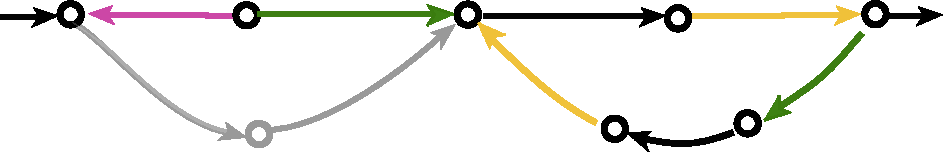
\includegraphics[scale=.45]{Pictures/encoding-set-of-paths.pdf}
 \end{center}
 \end{example}
  
 \begin{proposition}\label{prop:encoding-guarded-sets-of-paths}
 Let $G$ be a graph and $P$ a set of orthogonal paths of $G$. There is a footprint $\mathbb{F}$ such that $P$ is the set of paths encoded by $\mathbb{F}$.
\end{proposition} 
\begin{proof}
 We define $\mathbb{F}$ as the natural paths encoding associated to $P$: its path edges and path vertices are respectively the set of edges and vertices that appear in the paths of $P$, its frontier, inner, opening, closing and simple edges are the corresponding edges in the paths of $P$. Notice that it is possible reorient the edges of every path so that it becomes directed. Since the paths of $P$ do not share any edge, we can reorient their edges consistently in order to make them directed. We define direct edges as the path edges whose orientation did not change after this operation,  and inverse edges the remaining path edges.
\smallskip

It is clear that the paths of $P$ are encoded by $\mathbb{F}$, let us show that they are the only ones. We start by stating the following claim which follows from the definitions.
\begin{claim}\label{claim}
Let $p$ be a path in $P$ and $v$ a vertex of $p$. If $v$ is the source (w.r.t. the new orientation induced by $\mathbb{F}$) of an inner edge or the closing edge of $p$, then, by construction, $v$ cannot be an interface vertex of $p$. If $v$ is the target (w.r.t. the new orientation induced by $\mathbb{F}$) of an inner edge or the opening edge of $p$, then by construction, $v$ cannot be an interface vertex of $p$.
\end{claim}
Let $p$ be a path encoded by $\mathbb{F}$. If $p$ has a unique edge, then it is a single edge, and by construction single edges come exclusively from paths of $P$ with a unique edge. In this case, $p$ is clearly a path in $P$. 

Suppose now that $p$ has at least two edges. The opening edge of $p$ is, by construction, the opening edge of some path $q$ of $P$. Let $v$ be the vertex of $p$ such that all the vertices between the input of $p$ and $v$ are also vertices of $q$ and the successor of $v$ in $p$, call it $w$, is not a vertex of $q$. 

By Claim~\ref{claim}, and since $v$ is the target of the opening edge or an inner edge of the path $q$, it is not an interface vertex of $q$.

Let $e$ be the edge  from $v$ to $w$ in the path $p$. The edge $e$ is either an inner edge or a closing edge, and by construction, there is a path $r$ of $P$ containing this edge. By Claim~\ref{claim}, and since $v$ is the source of an inner edge or the closing edge of $r$, we have that $v$ is not an interface vertex of $r$. 

Here is a picture illustrating this construction, where the path between $\iota$ and $o$ is $p$.
\begin{center}
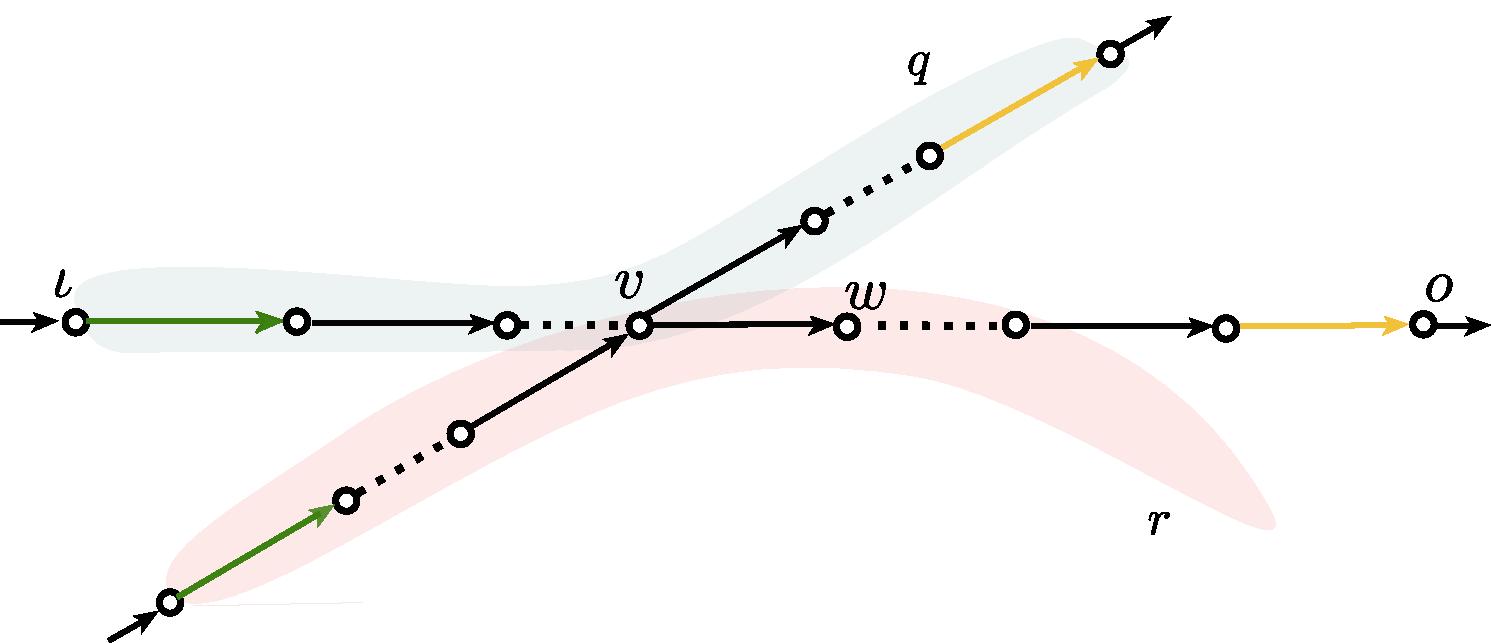
\includegraphics[scale=.3]{Pictures/proof-encoding-paths}
\end{center}
We have found two paths of $P$, $q$ and $r$, sharing a vertex $v$ which is an interface vertex of none of them. This yields a contradiction. 
\end{proof}

\begin{theorem}
If a language is $\CMSO^r$ definable then it is $\CMSO$ definable.
\end{theorem}

\begin{proof}
Let $\phi$ be a $\CMSO^r$ formula. We transfor $\phi$ into a $\CMSO$ formula $\psi$ as follows. We replace every quantification $\exists R.$ by a sequence of existential sets quantifications representing  a footprint $\mathbb{F}$. 

Saying that a subgraph $(s,Z,t)$ is a directed path is expressible in $\CMSO$, and checking that its different components (frontier vertices, opening and closing edges, etc) match the footprint is also easily expressible in $\CMSO$. Hence we can define a  $\CMSO$ formula $\mathsf{encoded\text{-}path}_\mathbb{F}(s,Z,t)$ which says that $(s,Z,t)$ is a path encoded by $\mathbb{F}$. 

We replace every  subformula of $\phi$ of the form ``$(s,t)\in R$'' by the following formula: $$\exists Z.\ \mathsf{encoded\text{-}path}_\mathbb{F}(s,Z,t)$$
\end{proof}

\section{Regular implies $\CMSO$ definable}\label{sec:reg->def}


\begin{theorem}\label{thm:reg->MSO}
If a language is regular, then it is $\CMSO$ definable. 
\end{theorem}

To prove Thm.~\ref{thm:reg->MSO}, we proceed by induction on  regular expressions. The cases of word and multiset regular expressions follow from the similar result for words and commutative words. The cases of union and the operations of the signature $\sigma$ follow from Prop.~\ref{prop:CMSO-def-operations}. We are left with the cases of substitution and iteration; the rest of this section is dedicated to proving the following proposition.
 
\begin{proposition}\label{prop:Guarded-It-Is-CMSO}
Let $x$ be a letter and $L$ and $M$ be languages of $\TWT$ graphs. We have:
$$
\begin{array}{ccc}
\text{$M [L/x]$ is guarded and $L$ and $M$ are $\CMSO$-definable} & \Rightarrow & \text{$M[L/x]$ is $\CMSO$-definable.}\\[3pt]
\text{$\mu x. L$ is guarded and $L$ is $\CMSO$-definable} &\Rightarrow& \text{$\mu x. L$ is $\CMSO$-definable.}
\end{array}$$
\end{proposition}


We handle the case of iteration, the case of substitution being similar. We show first that the iteration of a $\CMSO$ definable language, without any guard condition, is definable in an extension of $\CMSO$ where we are allowed to quantify existentially over sets of subgraphs of the input graph, which we call $\CMSOd$. This logic is obviously strictly more expressive then $\CMSO$, because it amounts to quantify over sets of sets. Based on this, we show that the  \emph{guarded iteration} of a $\CMSO$ definable language is  definable in $\CMSO^r$, the extension of $\CMSO$ with companion relations defined in the previous section. This concludes the proof, the logic $\CMSO^r$  being equivalent to $\CMSO$.



\subsection{Iteration of $\CMSO$ formulas is $\CMSOd$ definable}

\subsubsection{Decompositions}

When a graph is in the iteration $\mu x. L$ of some language $L$, it is possible to structure it into a tree shaped decomposition, such that each part of this decomposition ``comes from $L$''. In the following, we define such decompositions.  


\begin{definition}[Independent graphs] 
Let $G$ be a graph and $H, K$ be subgraphs of $G$.  We say that $H$ and $K$ are \emph{independent} if they do not share any edge; and whenever they share a vertex, it is necessarily an interface vertex of both $H$ and $K$. 
\end{definition}
\begin{remark}
Two independent subgraphs can share at most two vertices.
\end{remark}
\begin{definition}[Decompositions]
A \emph{decomposition} of $G$ is a set $\cD$  of modules of $G$ such that  $G\in \cD$ and for every pair of  graphs in $\cD$, they are either independent, or strict module one of the other. We call  the graphs of  a decomposition its \emph{components}. We call \emph{the interfaces of $\cD$} the set of interfaces of its components. 
\smallskip

Let $H$ and $K$ be components of a decomposition $\cD$. We say that $H$ is a \emph{child} of $K$, if $H$ is a module of $K$, and if there is no component $C$ of $\cD$, distinct from $H$ and $K$,  such that $H$ is a module of $C$ and $C$ is a module of $K$. 
\smallskip

The graph $G$ is called the \emph{head} of $\cD$. A component of $\cD$ is a \emph{leave} if it does not contain another component of $\cD$ as a module.
 \end{definition}
 \begin{remark} Note that  the children of a component are pairwise independent.
\end{remark}


 \begin{example}\label{example:decomposition} Let $G$ be the left graph below. The right picture is a decomposition of $G$, where the child relation  is materialized by the dotted lines. The colors have no specific meaning here, but will be useful to illustrate the upcoming notion of the \emph{components body}.  
 \begin{center}
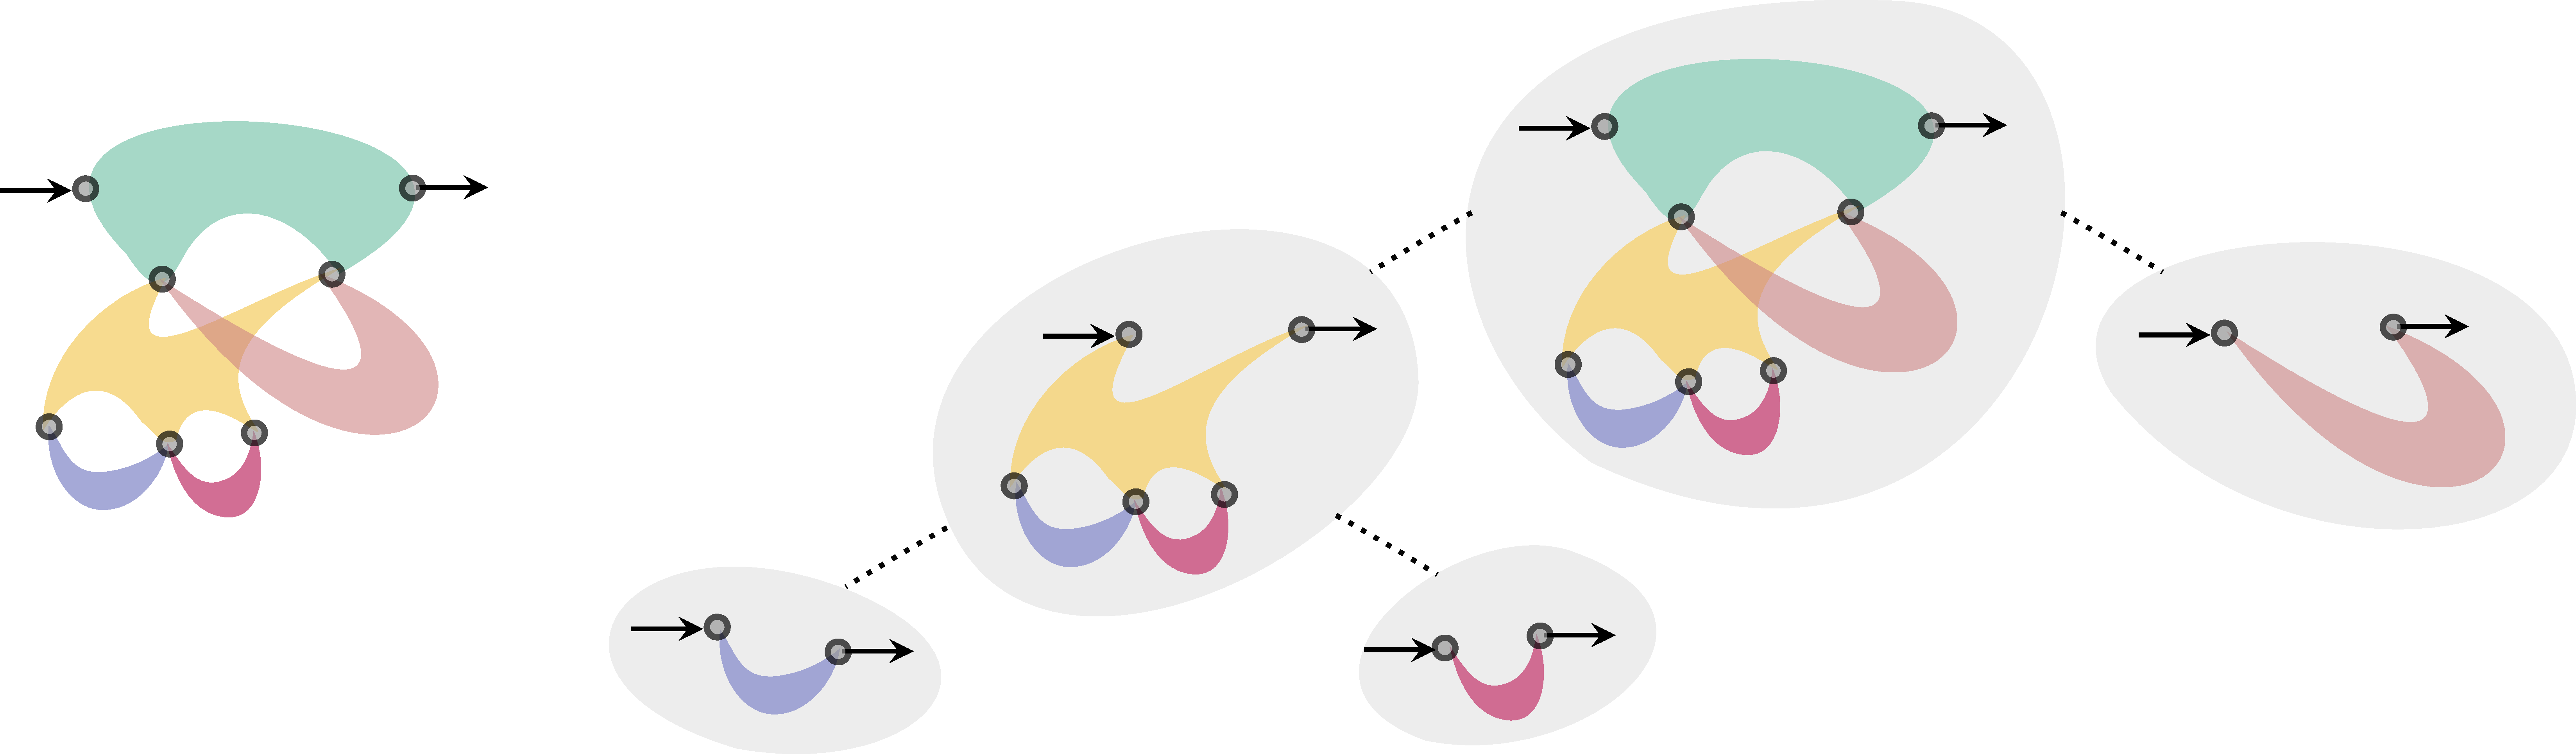
\includegraphics[scale=.10]{Pictures/decomposition}
\end{center}
 \end{example}
 
 \begin{definition}[Body of a component]
Let $G$ be a graph, $\cD$ a decomposition of $G$ and $C$ a component of $\cD$. 
\smallskip

The \emph{body} of $C$ is the subgraph of $G$ whose vertices are those of $C$ minus the \textbf{inner} vertices of its children; and whose edges are those of $C$ minus those of its children. We denote it by  $\mathsf{body}_\cD(C)$.  
\smallskip

The \emph{$x$-body of $C$} is the graph whose interface is the interface of $C$, whose vertices are the vertices of the body of $C$, and whose edges are the edges of the body of $C$ plus, for each child $F$ of $C$, an $x$-edge whose interface is the interface of $F$.  We denote it  by $x\text{-}\mathsf{body}_\cD(C)$.
\end{definition}

\begin{definition}[$L$-decompositions]
Let $L$ be a graph language. An $L$-decomposition of a graph $G$ is a decomposition of $G$ such that the $x$-body of each of its components is in $L$.
\end{definition}

\begin{example}
Below, from left to right, a component of the decomposition of Ex.~\ref{example:decomposition}, its body, and its $x$-body. Actually, each monochromatic subgraph of $G$ corresponds to the body of a  component of this decomposition.
\begin{center}
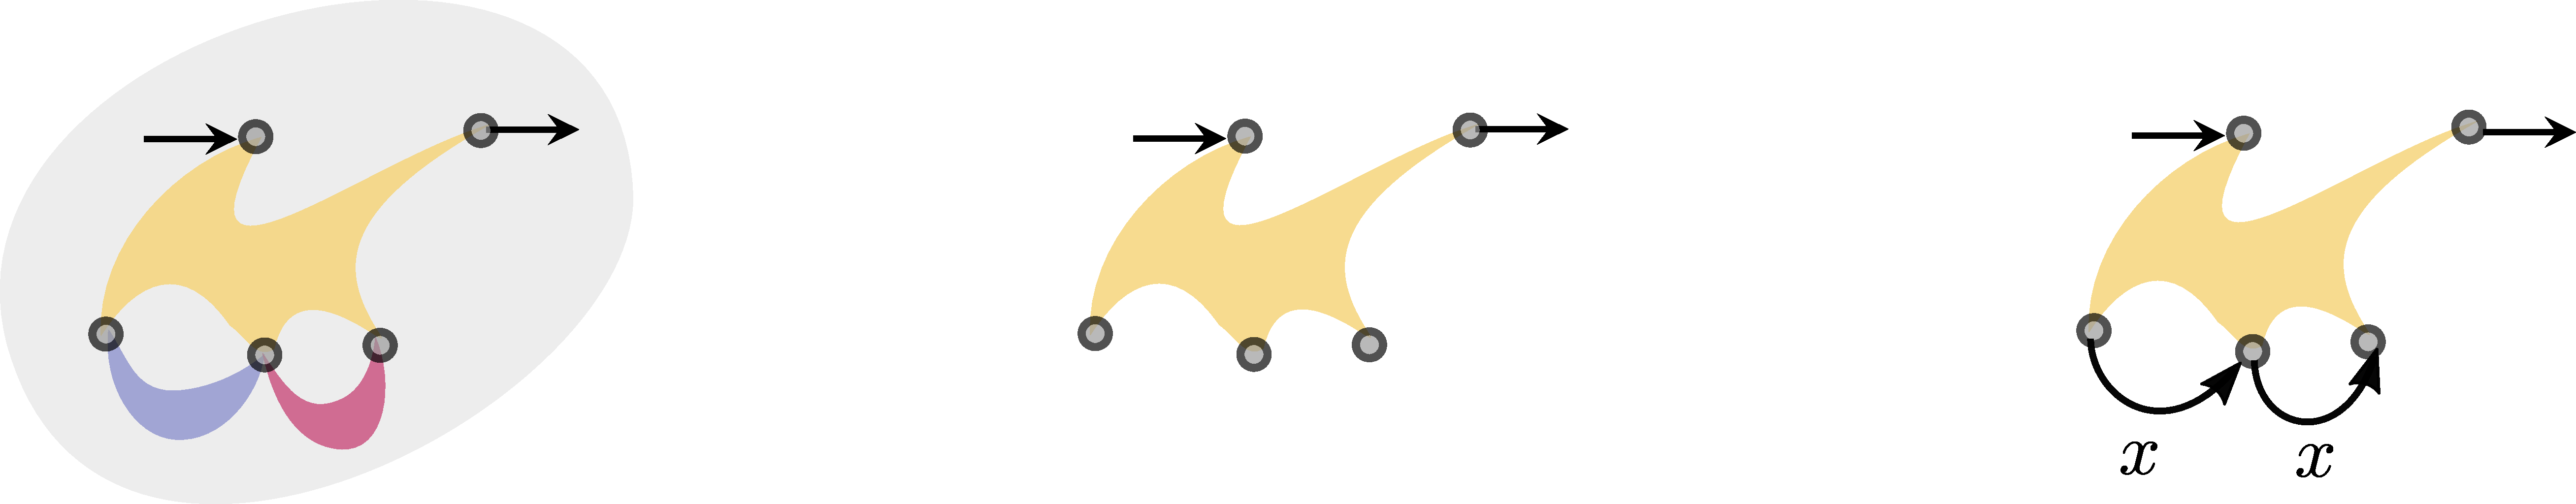
\includegraphics[scale=.10]{Pictures/body}
\end{center}
\end{example}
\begin{remark}
The body of a component is a subgraph of $G$, but its $x$-body is not a subgraph of $G$ in general, because of the added $x$-edges.
\end{remark}


 

\begin{proposition}\label{lem:decomp-iteration}
Let $L$ be a graph language. We have:
$$ G\in \mu x. L \qquad \Leftrightarrow \qquad \exists \cD. \ \quad\cD \text{ is an $L$-decomposition of $G$.}$$
\end{proposition} 
The proof of this proposition is based on the following easy lemma:

\begin{lemma}\label{lem:decomp-one-step}
Let $L$ be a language, $G, G_1,\dots, G_k$ be graphs and $H$ a $k$-context satisfying:
 $$G=H[G_1,\dots, G_k]\qquad\text{ and }\qquad H[x,\dots,x]\in L$$
Let $\cD_i$ be an $L$-decomposition for $G_i$, for $i\in [1,k]$, and let $\cD$ be the following set
 $$\cD:=\cD_1\cup \dots\cup \cD_k\cup\set{G}.$$
 The set $\cD$ is an $L$-decomposition of $G$.
\end{lemma}

\begin{proof}[Proof of Prop.~\ref{lem:decomp-iteration}]
We show by induction on $n\in\mathbb{N}$, that the  property $P_n$ is true:
$$\begin{array}{lrll}
P_n:&\qquad\forall G.\ \quad G\in L^{n,x}& \Rightarrow& \exists \cD. \ \quad\cD \text{ is an $L$-decomposition of $G$.} 
\end{array}
$$
The base case is trivial, and the inductive case is based on Lemma~\ref{lem:decomp-one-step}.
\end{proof}



\subsubsection{The logic $\CMSOd$}
Let $\phi$ be a $\CMSO$ formula defining a graph language $L$. Using Prop~\ref{lem:decomp-iteration}, we can express that a graph $G$ is in the iteration $\mu x. L$ by guessing a decomposition $\cD$ of $G$, and ensuring that the $x$-body of each component  satisfies $\phi$.   But guessing a set of subgraphs is not expressible in $\CMSO$. This is why we introduce $\CMSOd$, an extension of $\CMSO$ where this is allowed. 


\begin{definition}[$\CMSOd$ logic] Let $\mathbb{X}_d$ be a set of \emph{graph set variables}, whose elements are denoted $\cX, \cY\dots$. The formulas of $\CMSOd$ are of the following form:
\begin{align*}
 \phi :=&\ \CMSO\ |\ \exists \cX.\ \phi\ |\ (s,Z,t)\in \cX & \qquad (\cX\in \mathbb{X}_d, \ \ Z\in \mathbb{X}_2,\ \  s,t\in\mathbb{X}_1).
\end{align*}
\end{definition}
Free and bound variables are defined as usual.  As for $\CMSO$, we need to define the semantics of a formula over pointed graphs to handle free variables. 

\begin{definition}[Semantics of $\CMSOd$] Let $G$ be a graph and $\Gamma$ be a set of variables.  

An \emph{interpretation of $\Gamma$} is a function mapping every first-order variable of $\Gamma$ to an edge or vertex of $G$, every set variable to a set of edges and vertices of $G$, and every graph set variable to a set of subgraphs of $G$.    

We define the \emph{satisfiability relation} $\langle G, I\rangle\models \phi$ as usual, by induction on  $\phi$. The only new cases compared to $\CMSO$ are the quantification  $\exists \cX$ which is interpreted as ``there exists a set of subgraphs $\cX$'', and the formulas $(s,Z,t)\in \cX$ which are interpreted as ``the graph whose input is $s$, whose output is $t$ and whose set of edges and vertices is $Z$, is an element of $\cX$''.  
\end{definition}
\begin{proposition}\label{prop:def-decomp}
There is a $\CMSOd$ formula $\mathsf{decomp}(\cX)$, \emph{without graph set quantification}, such that for every graph $G$ and every set of subgraphs $\cD$ of $G$, we have:
\begin{align*}
\qquad\qquad\qquad\langle G, \cX\mapsto \cD\rangle\models \mathsf{decomp}(\cX)\quad \Leftrightarrow \quad  \cD \text{ is a decomposition of } G.
\end{align*}
\end{proposition}
\begin{proof} 
We can express in $\CMSOd$ that a graph is a module of another graph using Prop.~\ref{prop:pure-modules-are-CMSO}. We can express that two graphs $(s,Z,t)$ and $(s',Z',t')$ are independent using the following formula:
$$ (x\in Z\  \wedge\  x\in Z')\ \ \Rightarrow (x=s\  \vee\  x=s'\  \vee\  x=t\ \vee\ x=t')$$
 This is how we express that $\cX$ is a decomposition. Note that we do not need to introduce a  quantification on new graph set variables. 
\end{proof}


\subsubsection{Iteration is expressible in $\CMSOd$}

Given a $\CMSO$ formula $\phi$, we construct a formula $\tms{\phi}$ having $\cX$ as unique free variable, which expresses the fact that the $x$-body the head of the decomposition $\cX$ satisfies $\phi$. To construct $\tms{\phi}$, we need the following definition.

\begin{definition}[Complete sets] Let $\cD$ be a decomposition of a graph $G$. 
\smallskip

Let $H$ be a set of edges and vertices of $G$. We say that $H$ is \emph{complete} if, whenever it contains an edge or an inner vertex of a child $C$ of $G$ (seen as a component of $\cD$), then it contains all the edges and  inner vertices of $C$. 
\smallskip

Let $K$ be a set of edges and vertices of the $x$\text{-}body of $G$.  We denote by $\mathsf{completion}_\cD(K)$ the set of edges and vertices of $G$,  obtained from $K$ by replacing every $x$-edge coming from a child $C$ of $G$  by the set of edges and inner vertices $C$.  
\end{definition}
\begin{remark}
Note that if $H$ is complete, there is a set $S$ such that $H=\mathsf{completion}_\cD(S)$.
\end{remark}

Here is a picture illustrating complete sets. The green part is the body of $G$ and the purple modules are its children. The yellow sets are complete, but the pink one is not. 
\begin{center}
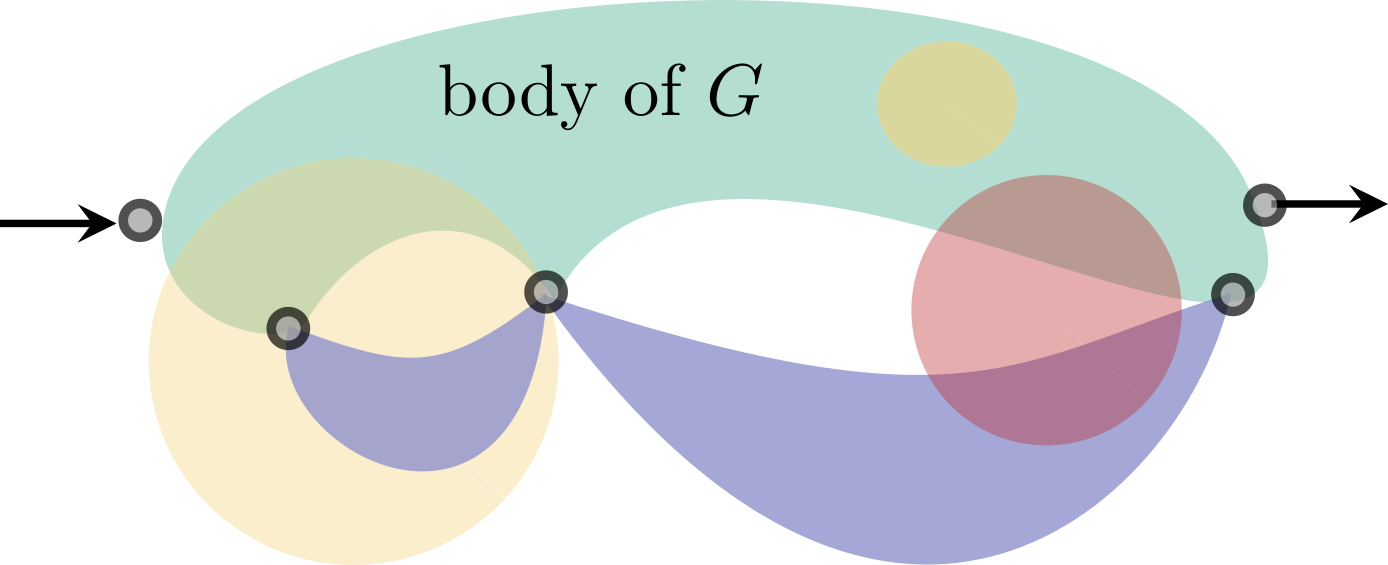
\includegraphics[scale=.12]{Pictures/complete-set}
\end{center}

\begin{proposition}
There are $\CMSO$ formulas $\mathsf{child}_\cX(Y)$, $\mathsf{complete}_\cX(Y)$, $\mathsf{body\text{-}edge}_\cX(Y)$, $\mathsf{source}_\cX(Y,Z)$, $\mathsf{target}_\cX(Y,Z)$ and $\mathsf{choice}_\cX(Y,Z)$ such that, for every graph $G$, every decomposition $\cD$, every subsets $H$ and $K$ of the edges and the vertices of $G$, we have the following, where  we write, by abuse of notation, $\mathsf{child}_\cD(H)$ instead of $\langle G, \cX\mapsto \cD, Y\mapsto H\rangle\models \mathsf{child}_\cX(Y)$ etc:\\
\noindent \begin{flushleft}
\begin{tabular}{llp{10cm}} 
$ \mathsf{child}_\cD(s,H,t)$&$\Leftrightarrow$& $s, t\notin H$ and $(s,H\cup\set{s,t},t)$ is a child of $G$ w.r.t.  $\cD$.\\[10pt]
$\mathsf{child}_\cD(H)$&$\Leftrightarrow$& $H$ is the set of edges and inner vertices of a child of $G$ w.r.t.  $\cD$.\\[10pt]
 $ \mathsf{complete}_\cD(H)$ &$\Leftrightarrow$&  $H$ is complete w.r.t. $\cD$.\\[10pt]
 $\mathsf{body\text{-}edge}_\cD(H)$&$\Leftrightarrow$& $H$ is a singleton containing an edge from  $\mathsf{body}_\cD(G)$.\\[10pt]
 $ \mathsf{source}_\cD(H,K)$&$\Leftrightarrow$& there are vertices  $ s$ and $t$ of $G$ such that $H=\set{s}$  and   $\mathsf{child}_\cD(s,K,t)$.\\[10pt]
 
 $\mathsf{target}_\cD(H,K)$&$\Leftrightarrow$ &there are vertices  $ s$ and $t$ of $G$ such that $H=\set{t}$  and   $\mathsf{child}_\cD(s,K,t)$.\\[10pt]
  $\mathsf{choice}_\cD(H,K)$&$\Leftrightarrow$ & $H$ is complete,  $K$ contains $\mathsf{body}_\cD(G)\cap H$, and contains exactly one edge of each  child of $G$  contained in $H$.
\end{tabular}
\end{flushleft}
\end{proposition}


\begin{proof}
We define the formulas of the proposition as follows. The formulas between quotation marks are not primitives of $\CMSO$ but can be  easily defined by $\CMSO$ formulas. 
 \begin{align*}
\mathsf{child}_\cX(x,Y,y)\ := \ \neg(x\in Y)\ \wedge\ &  \neg(y\in Y)\ \wedge\  \exists Z.\ (\text{``$Z=Y\cup\set{x,y}$''} \ \wedge\ (x,Z,y)\in \cX ) \\
\wedge\ \big(\ \forall Z'. \forall x', \forall y'.&\ (x',Z', y')\in \cX \wedge \text{``$(x,Z,y)$ is a module of $(x',Z',y')$''}\\
                    & \Rightarrow\ \text{``$(x',Z',y')$ is the whole graph.''}\ \big)
\end{align*} 
$$ 
\begin{array}{lll}
\mathsf{child}_\cX(Y) &:= &  \exists x.\ \exists y.\ \mathsf{child}_\cX(x,Y,y) \\[10pt]
\mathsf{complete}_\cX(Y)& := &  (\exists Z.\ \exists x.\ \mathsf{child}_\cX(Z)\ \wedge\ \text{``$x\in Y\cap Z$''} )\ \ \Rightarrow\ \ (Z\subseteq Y) \\[10pt]
 \mathsf{body}_\cX(x) &:= &\forall Z.\ \ \mathsf{child}_\cX(Z)\ \Rightarrow\ \neg(x\in Z) \\[10pt]
 \mathsf{body\text{-}edge}_\cX(Y)& :=& \exists x.\ \text{``$Y=\set{x}$''} \ \wedge \ \mathsf{body}_\cX(x)\\[10pt]
 \mathsf{choice}_\cX(Y,Z)&:=& \ \mathsf{complete}_\cX(Y)\ \wedge \ \forall x.\ (x\in Y)\wedge \mathsf{body}_\cX(x)\ \Rightarrow\ (x\in Z)\ \\
 && \wedge\ \forall C.\ \mathsf{child}_\cX(C)\ \wedge \ (C\subseteq Y) \Rightarrow\ 
 \text{``$\exists!  x\in (C\cap Z)$''}    
\end{array}
$$
The formula $ \text{``$\exists!  x\in (C\cap Z)$''}$ is the following:
$$ \exists x.\ \text{``$(x\in C\cap  Z)$''}\wedge \forall y.\ \text{``$(y\in C\cap Z)$''} \ \Rightarrow \ (y=x)$$
 \end{proof}
%\begin{remark}
%Pour construire $\mathsf{choice}_\cX(Y,Z)$, nous avons besoin que les elements de la decomposition ne soient pas vides. 
%\end{remark}
 We construct the formula $\tms{\phi}$ by induction on the structure of $\phi$. We suppose that $\phi$ is build using the syntax of $\CMSO$ where only set variables are allowed.

\begin{definition}\label{def:transfer}  Let $\phi$ be a $\CMSO$ formula whose free variables are $\Gamma$. 
 We define the $\CMSOd$ formula $\tms{\phi}$, whose free variables are $\Gamma\cup\set{\cX}$,  by induction as follows:
 $$\begin{array}{lll}
    \tms{\phi\vee \psi}&= & \tms{\phi} \vee \tms{\psi} \\[4pt]
    \tms{\neg \phi}&= & \neg \tms{\phi}\\[4pt]
      \tms{(|Y|\equiv k)[m]}&= & \exists Z.\ \mathsf{choice}_\cX(Y,Z)\wedge (|Z|\equiv k)[m]\\[4pt]
   \tms{Y\subseteq Z}&= & Y\subseteq Z \\[4pt]
    \tms{\mathsf{input}(Y)}&= &  {\mathsf{input}(Y)}\\[4pt]
     \tms{\mathsf{output}(Y)}&= &  {\mathsf{output}(Y)}\\[4pt]
     \tms{a(Y)}&= & a(Y)\qquad (a\neq x) \\[4pt]
       \tms{x(Y)}&= & \mathsf{child}_\cX(Y) \vee (\mathsf{body\text{-}edge}_\cX(Y)\wedge x(Y) ) \\[4pt]
        \tms{\exists Y.\ \phi}&= &\exists Y.\ \mathsf{complete}_\cX(Y)\wedge \tms{\phi}\\[4pt]
 \tms{\mathsf{source}(Y,Z)}& =&(\mathsf{body\text{-}edge}_\cX(Z)\wedge \mathsf{source}(Y,Z) )\vee (\mathsf{child}_\cX(Z)\wedge \mathsf{source}_\cX(Y,Z) )\\[4pt]
 \tms{\mathsf{target}(Y,Z)}&= &(\mathsf{body\text{-}edge}_\cX(Z)\wedge \mathsf{target}(Y,Z) )\vee (\mathsf{child}_\cX(Z)\wedge \mathsf{target}_\cX(Y,Z) )
 \end{array}
 $$
 \end{definition}

Transfer results are results of this form: to check that a transformation $\mathsf{f}(G)$ of a structure $G$ satisfies a formula $\phi$, construct a formula $\mathsf{f}^{-1}(\phi)$ that $G$ should satisfy. The proposition below is a transfer result, where the transformation is the $x$-body.

 \begin{proposition}\label{prop:transfer}
Given a $\CMSO$ sentence $\phi$ defining, there is a $\CMSOd$ formula $\tms{\phi}$ having $\cX$ as unique free variable, such that for every graph $G$ and every decomposition $\cD$  of $G$ \emph{whose components are non-empty}:
$$\langle G,\cX\mapsto\cD\rangle \models\tms{\phi}\qquad \Leftrightarrow \qquad  \text{$x$-}\mathsf{body}_\cD(G)\models \phi.$$
\end{proposition}



\begin{proof} We start by the following definition.
\begin{definition} Let  $\cD$ be a decomposition of  $G$ and $I$  an interpretation of the  set variables $\Gamma$ in  the $x$-body of $G$. We define $I_\cD$, the interpretation of $\Gamma\cup\set{\cX}$ in  $G$ as follows.
\begin{align*}
\qquad\qquad \qquad \quad I_\cD:\ \ & \cX \mapsto \cD, \\
      &   Y \mapsto \mathsf{completion}_\cD(I(Y)), \quad Y\neq \cX.
\end{align*} 
\end{definition}
Let $G$ be the left graph below, the purple graphs being its children for a decomposition $\cD$. The right graph is its $x$-body. The right yellow circles represent the interpretation $I$ of the variables $Y$ and $Z$ in the $x$-body. The left yellow circles represent the interpretation $I_\cD$ of these variables in $G$. 
\begin{center}
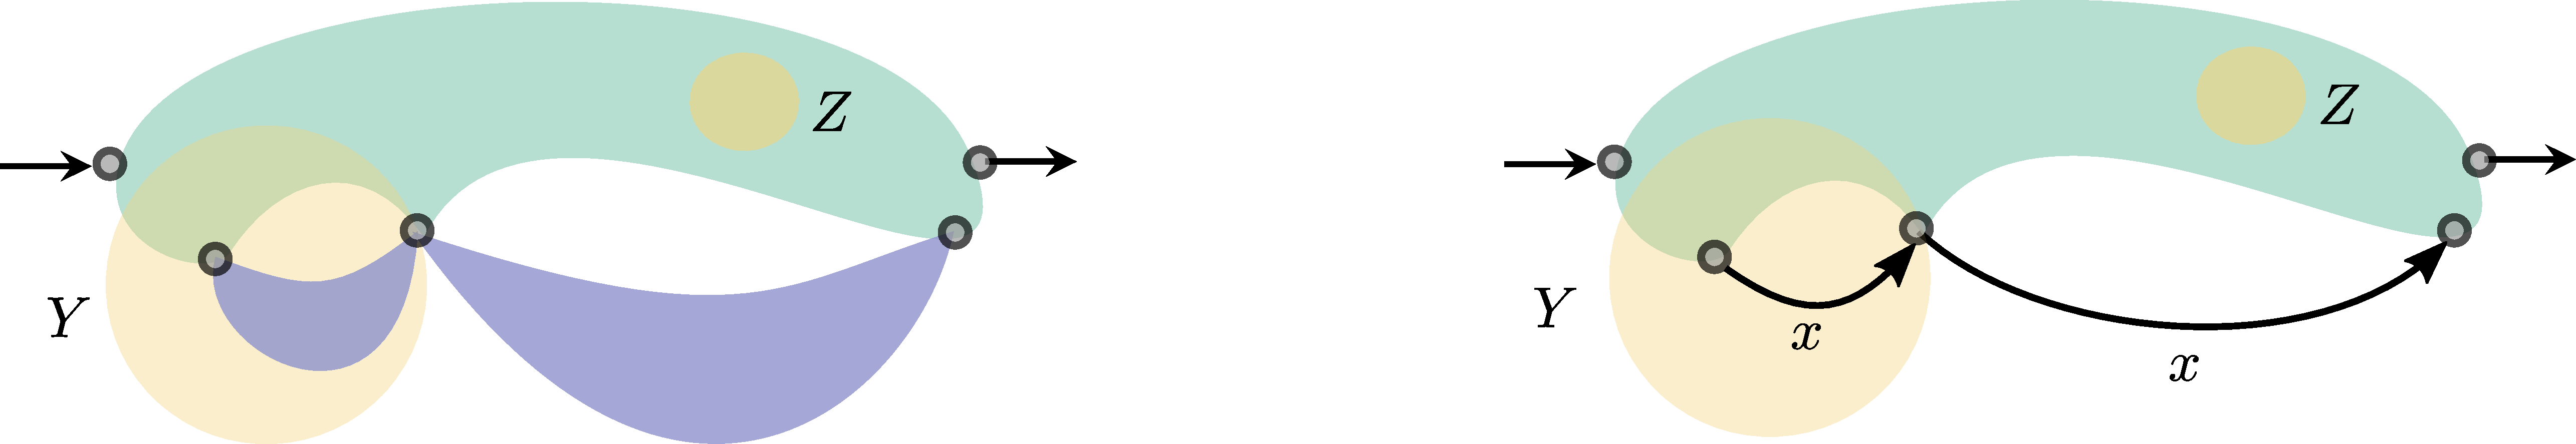
\includegraphics[scale=.12]{Pictures/transfer-interpretation}
\end{center}
The following lemma, which generalizes Prop.~\ref{prop:transfer}, can be proved by a straightforward induction, concluding the proof of this proposition.
 \begin{lemma}
 Let $\cD$ be a decomposition of $G$, $\phi$ a $\CMSO$ formula whose variables are $\Gamma$ and $I$ an interpretation of  $\Gamma$ in the $x$-body of $G$. We have:
 $$ \langle G, I_\cD\rangle \models \tms{\phi} \qquad \Leftrightarrow \qquad\langle x\text{-}\mathsf{body}_\cD(G), I\rangle \models \phi$$ 
 \end{lemma}
We added the non-emptiness condition on the components of $\cD$ to handle the case where $\phi=(|Y|\equiv k)[m]$.
 \end{proof}

The formula  $\tms{\phi}$ expresses the fact that the $x$-body of the head of a decomposition satisfies $\phi$. Using this formula and the localization construction of Prop.~\ref{prop:localization}, we construct a formula $\mu x. L$ saying that the $x$-body of \textbf{all} the components of a decomposition satisfy $\phi$.

\begin{definition}\label{def:iteration}
If $\phi$ is a $\CMSO$ formula, we let $\mu x. \phi$ be the following $\CMSOd$ formula: $$\mu x. \phi:=\ \exists\cX.\ \mathsf{decomp}(\cX)\ \ \wedge\ \ \forall s. \forall Z.\ \forall t.\ (s,Z,t)\in\cX\ \Rightarrow\ \tms{\phi}|_{(s,Z,t)}$$
\end{definition}
The following proposition says that  the language of $\mu x. \phi$ is the iteration of that of $\phi$. 
\begin{proposition}\label{prop:lang-iteration} If $\phi$ is a $\CMSO$ formula defining a language of non-empty graphs, then: $$\ \cL(\mu x. \phi)=\mu x. \cL(\phi).$$
\end{proposition}
\begin{proof} Let $[\phi]$ be the following formula:
$$[\phi]\ :=\ \forall s.\forall Z.\ \forall t.\ \ (s,Z,t)\in\cX\ \Rightarrow\  \tms{\phi}|_{(s,Z,t)}$$  By Prop.~\ref{prop:transfer} and Prop.~\ref{prop:localization}, we can prove the following lemma:
\begin{lemma}
For every graph $G$ and every decomposition $\cD$ of $G$:
$$\langle G,\cX\mapsto\cD\rangle \models[\phi]\qquad \Leftrightarrow \qquad  \forall C\in \cD, \ \text{$x$-}\mathsf{body}_\cD(C)\models \phi.$$
\end{lemma}
We conclude the proof by Prop.~\ref{lem:decomp-iteration}.
\end{proof}

\begin{corollary}
If $L$ is $\CMSO$ definable then  $\mu x. L$ is $\CMSOd$ definable.
\end{corollary}

\subsection{Guarded iteration of $\CMSO$ languages is $\CMSO^r$ definable}

The idea here is that when the iteration $\mu x. L$ is guarded, $L$-decompositions can be encoded by sets of edges and vertices and by companion relations.

\subsubsection{The case of  test languages}
Let $\mu x. L$ be a guarded iteration of type \emph{test}, $G\in \mu x. L$ and $\cD$ an $L$-decomposition of $G$. Suppose that $G$ is the left graph below, and that the red vertices are the interfaces\footnote{Recall that test graphs are unary, hence all the components of a decomposition of $G$ are unary.} of $\cD$.
\begin{center}
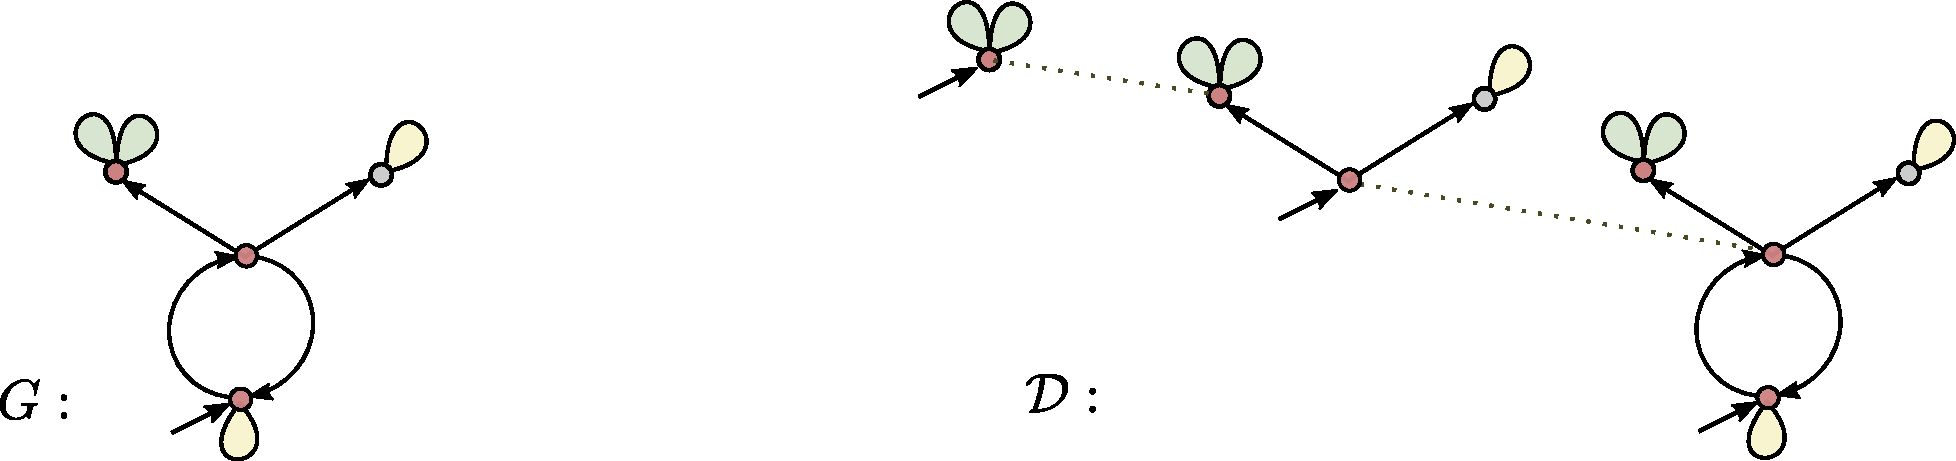
\includegraphics[scale=.33]{Pictures/decomp-test}
\end{center}
We claim that, thanks to the guard condition, this information is enough to reconstruct the whole decomposition $\cD$. More precisely, we claim that the components of $\cD$ are exactly the maximal modules of $G$, whose interfaces are the red vertices, as depicted above.

%This decomposition is depicted above.  By definition, a component of $\cD$ is a module of $G$ whose interface is a red vertex. What we need to show is its maximality. 

%To give an idea for why this should be the case, consider the following decomposition $\cD'$ where one of the components, called $M$, is \textbf{not} a maximal module. Let $H$ be  the $x$-body of $G$ with respect to the decomposition $\cD'$. Notice that  $x$ has a parallel face in $H$, which is not possible because of the guard condition and because  $H\in L$.
%\begin{center}
%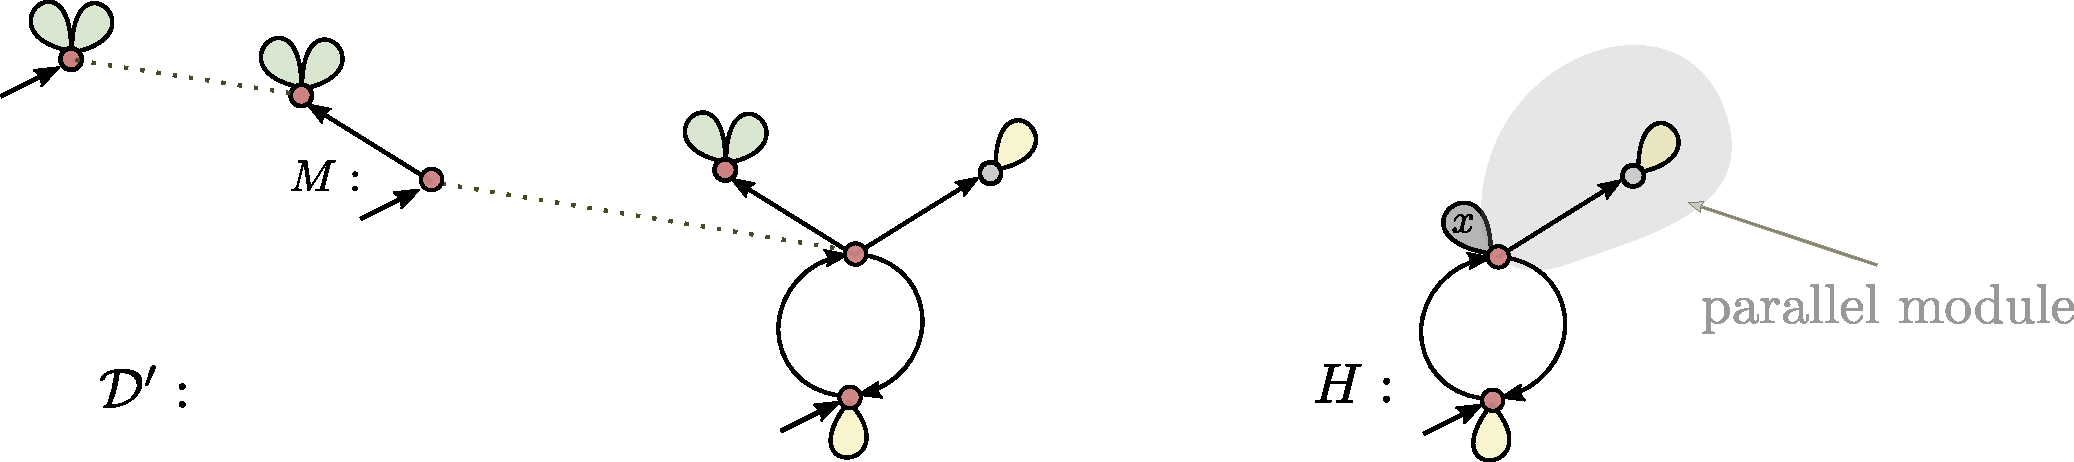
\includegraphics[scale=.4]{Pictures/if-not-max}
%\end{center}
%Our goal will be to make this idea more precise, and this justifies the following definition.
% which associates to a set of vertices of a given graph,  the maximal (unary) modules having these vertices as interfaces.


\begin{definition}  Let $G$ be a graph and $S$ be a set of vertices of $G$.   
We define $\cD_\mathsf{t}(S)$ as the set of maximal modules of $G$, whose type is test, and whose interfaces belong to $S$.  
\end{definition}

\begin{proposition}\label{prop:decomp-iteration-test} Let  $\mu x. L$ be a guarded iteration of type test. We have:
$$\begin{array}{rll}
  G\in \mu x. L& \qquad\Leftrightarrow \qquad\qquad& \exists S.\quad  S \text{ is a set of vertices of $G$ and }\\[3pt]
                      &             & \qquad \ \cD_\mathsf{t}(S) \text{ is an $L$-decomposition of $G$.} 
\end{array}
$$
\end{proposition}

\begin{proof} 
 $(\Rightarrow)$ Follows from Prop.~\ref{lem:decomp-iteration}. To prove  $(\Leftarrow)$, we define the property $P_n$ as follows:
$$\begin{array}{lrll}
P_n:&\qquad\forall G.\ \quad G\in L^{n,x}& \Rightarrow& \exists S.\quad  S \text{ is a set of vertices of $G$ and }\\
 &                      &             & \qquad \cD_\mathsf{t}(S) \text{ is an $L$-decomposition of $G$.} 
\end{array}
$$
We prove, by induction on $n$, that $P_n$ is valid for every $n\geq 1$, and this is enough to conclude. 
\medskip

 When $n=1$, take $S$ to be the singleton containing the interface of $G$. We have that $\cD_\mathsf{t}(S)=\set{G}$ and since $G\in L$, we have that $\cD_\mathsf{t}(S)$ is an $L$-decomposition of $G$.
\medskip

 Let $G\in L^{n+1,x}$. By definition, there is a $k$-context $H$ and  graphs $G_1, \dots, G_k$ such that: 
$$G=H[G_1,\dots, G_k],\quad H[x,\dots,x]\in L\quad \text{ and }\quad G_i\in L^{n,x}, \text{ for } i\in[1,k].$$ 

Thanks to the guard condition, there is no module of $H$ parallel to a hole of $H$.  For every $i\in[1, k]$, let $S_i$ be the set of vertices provided by the induction hypothesis applied to the graph $G_i$. Here is a picture illustrating these notations:
\begin{center}
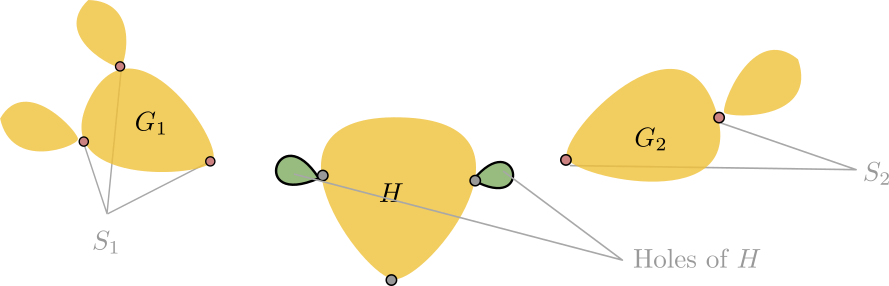
\includegraphics[scale=.36]{Pictures/decomp-test-proof}
\end{center}
By Lemma~\ref{lem:decomp-one-step}, the set of subgraphs $\cD$ defined below is an $L$-decomposition of $G$.
 $$\cD:=\cD_\mathsf{t}(S_1)\cup\dots\cup\cD_\mathsf{t}(S_k)\cup\set{G}$$
  To conclude we only need to find a set of vertices $S$ of $G$ such that $\cD_\mathsf{t}(S)=\cD$. Let $S=S_1\cup\dots\cup S_k\cup\set{\iota}$, where $\iota$ is the interface of $G$. Let us show that $\cD_\mathsf{t}(S)=\cD$. This is a consequence of the following lemma:

\begin{lemma}\label{lem-max-modules-context} Let $C$ be a context, $K$ a graph  and $I$ an interface in $K$ of the same arity as the hole of $C$. Suppose that the hole of $C$ is not parallel to any module. We have:
$$ \mathsf{max\text{-}module}_{\;C[K]}(I)=\mathsf{max\text{-}module}_{\;K}(I)$$
\end{lemma}
\begin{proof} Let $M:=\mathsf{max\text{-}module}_K(I)$.
Note that $M$ is a module of $G[K]$,  the question is its maximality. 
If $I$ is not the interface of $K$, then $M$ is maximal in  $G[K]$ because this substitution does not add any modules to $M$. 
Suppose that $I$ is the interface of $H$. In this case, we have $M=K$. Suppose by contradiction that there is a module $M'$ of  $G[K]$ strictly  containing  $K$ and whose interface is $I$. Hence, there is a module $M''$ such that $M'=(K\parallel M'')$. This means that $M''$ is module parallel to the hole of  $C$, which is not possible by hypothesis. 
\end{proof}
\end{proof}


\begin{theorem} 
Suppose that $\mu x. L$ is a guarded iteration of type test. We have: 
$$ L\text{ is $\CMSO$ definable} \quad \Rightarrow \quad  \mu x.L \text{ is  $\CMSO$ definable}$$
\end{theorem}

\begin{proof} Let $\phi$ be a $\CMSO$ formula whose language is $L$.
We transform the $\CMSOd$ formula $\mu x. \phi$ of Def.~\ref{def:iteration}, whose language is $\mu x. L$, into a $\CMSO$ formula  ${\mu x^g. \phi}$ of the same language. The formula ${\mu x^g. \phi}$ is obtained by replacing the quantification $\exists \cX.\ $ by the set quantification $\exists S.\ $, and by replacing every sub-formula of $\mu x. \phi$ of the form $(s,Z,t)\in \cX$ by this formula: 
$$(s=t) \ \wedge\ s\in S \ \wedge\ \text{``$(s,Z,t)$ is a maximal module''} $$
The last part of this formula is expressible in $\CMSO$ thanks to Prop.~\ref{prop:pure-modules-are-CMSO}. The language of ${\mu x^g. \phi}$ is the set of graphs for which we can find an $L$-decomposition encoded by a set of vertices $S$, and this is precisely the language $\mu x. L$ thanks to Prop.~\ref{prop:decomp-iteration-test}.
\end{proof}

\subsubsection{The case of domain  languages}
Let $\mu x. L$ be a guarded iteration of type \emph{domain}, $G$ a graph of $\mu x. L$ and $\cD$ an $L$-decomposition of $G$. Contrarily to the test case, the set of vertices  of $G$ corresponding to the interfaces of $\cD$, are not enough information to reconstruct $\cD$. Indeed, in this case,  a component of $\cD$ whose interface is $v$ is not necessarily the maximal module at $v$, but some domain module of interface $v$, among possibly many others. 
A way to determine if a domain module is in the decomposition is to check whether it contains an interface of the decomposition. This works for the components which are not the leaves of the decomposition. For the other components, we need to say explicitly which domain modules are the leaves. Since the later are pairwise independent, we can do so by coloring their inner edges and vertices. 



In the following, we show that a set of vertices of a graph (representing the interfaces of a decomposition) together with a coloring of this graph (indicating which modules are leaves), is enough to recover the decomposition. This justifies the following definitions.
 
\begin{definition}[Coloring, Active modules]
A \emph{coloring} of a graph $G$ is a set of its edges called \emph{leaf edges}. A module of $G$ is \emph{active} if it contains a leaf edge.

% A module is \emph{residual} if all its edges and inner vertices are residual; and \emph{principal} otherwise.
%
%\noindent Let $I$ be a pair of vertices in a graph. The \emph{maximal residual module at $I$} is the largest residual module whose interface is $I$.
\end{definition}
%\begin{remark}
%A module is principal if it contains \textbf{some} non-residual edge or  inner vertex.
%\end{remark}
%Given a set of vertices  $S$ and a coloring $\col$ of a graph $G$, we associate them with a set of subgraphs $\cD_\mathsf{d}(S, \col)$ as follows. 

\begin{definition}[$\cD_\mathsf{d}(S, \col)$] Let $G$ be a graph, $S$ a set of vertices and $\col$ a coloring of $G$.   

 \noindent We let $\cD_\mathsf{d}(S, \col)$ bet the set of active modules of $G$ of type $\mathsf{d}$, whose interfaces belong to $S$. 
\end{definition}

\begin{example} Consider the graph $G$ below, let $S$ be the set of red vertices and let $\col$ be the set containing the green edge. The decomposition $\cD$ below is $\cD_\mathsf{d}(S,\col)$.
\begin{center}
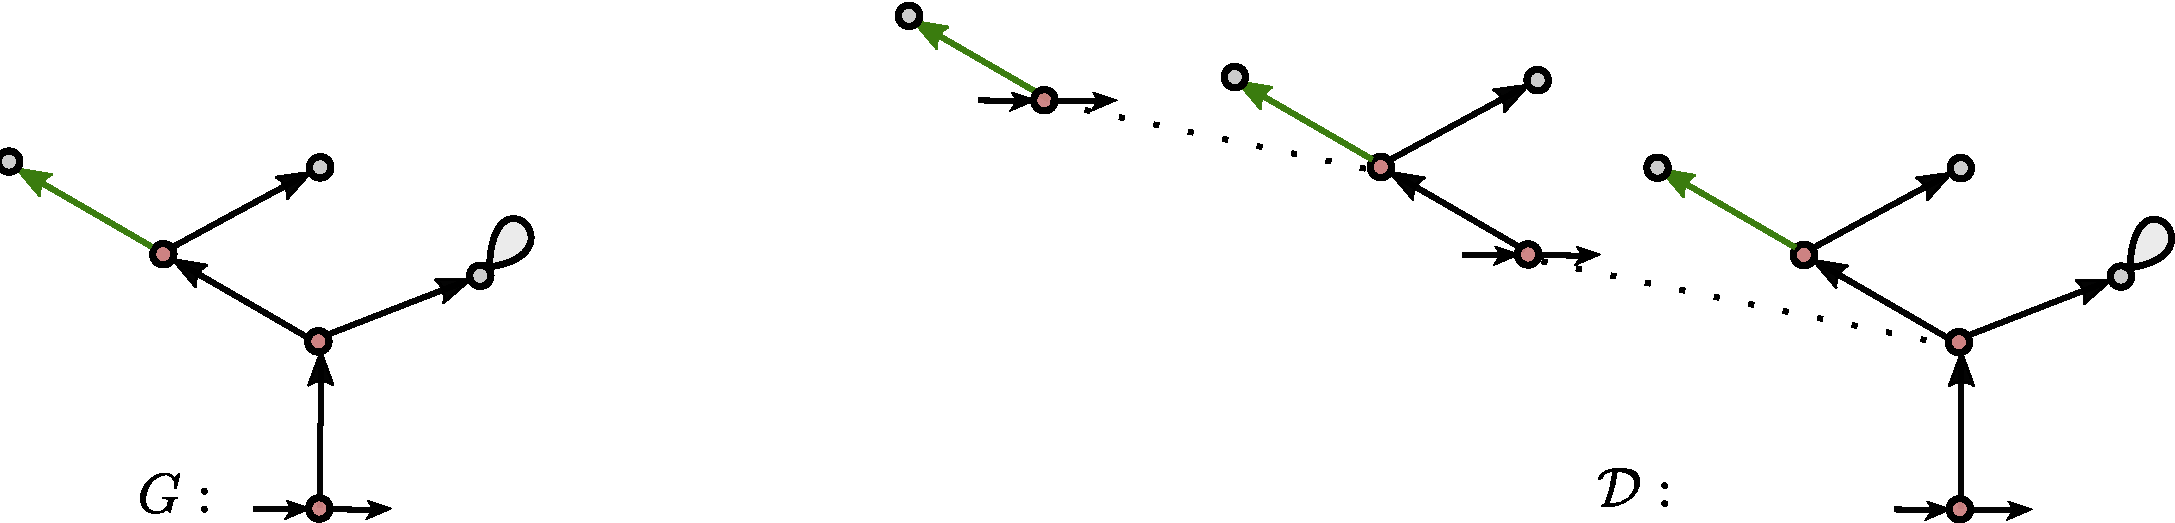
\includegraphics[scale=.33]{Pictures/decomp-dom}
\end{center}
\end{example}

\begin{proposition}\label{prop:decomp-iteration-dom} Let $L$ be  a domain language and $\mu x. L$ a guarded iteration. We have:
$$\begin{array}{rll}
 \quad G\in \mu x. L& \Leftrightarrow& \exists S, \col.\quad  S \text{ is a set of vertices and $\col$ a coloring of $G$ such that }\\
                      &             & \qquad\qquad \cD_\mathsf{d}(S,\col) \text{ is an $L$-decomposition of $G$.} 
\end{array}
$$
\end{proposition}

\begin{proof} 
The implication $(\Leftarrow)$ follows from Prop.~\ref{lem:decomp-iteration}. Let us prove the implication $(\Rightarrow)$.  Let $P_n$ be the following property:
$$\begin{array}{lrll}
P_n:&\ \forall G.\  G\in L^{n,x}& \Rightarrow& \exists S, \col.\quad  S \text{ is a set of vertices and $\col$ a coloring of $G$ such that }\\
 &                      &             & \qquad\qquad \cD_\mathsf{d}(S,\col) \text{ is an $L$-decomposition of $G$.} 
\end{array}
$$
We prove, by induction on $n$, that $P_n$ is valid for every $n\geq 1$, which  is enough to conclude. 
\medskip

 When $n=1$, we let $S$ be the singleton containing the interface of $G$ and  $\col$ be the coloring where all the edges of $G$ are leaves. We have $\cD_\mathsf{d}(S,\col)=\set{G}$, and since $G\in L$,   $\cD_\mathsf{d}(S,\col)$ is an $L$-decomposition of $G$.
\medskip

 Let $G\in L^{n+1,x}$. There are graphs $G_1, \dots, G_k$ and a $k$-context $H$ satisfying:
 $$G=H[G_1,\dots, G_k], \quad H[x,\dots,x]\in L\quad \text{ and }\quad  G_i\in L^{n,x} \text{ for } i\in[1,k].$$
 Let $S_i$ and $\col_i$ be the set of vertices and the coloring provided by induction hypothesis applied to $G_i$, for $i\in[1,k]$. 
 By Lemma~\ref{lem:decomp-one-step}, the set of subgraphs
 $$\cD:=\cD_\mathsf{d}(S_1,\col_1)\cup\dots\cup\cD_\mathsf{d}(S_k,\col_k)\cup\set{G}$$
 is an $L$-decomposition of $G$. To conclude we only need to find a set of vertices $S$ and a coloring $\col$ of $G$ such that $\cD_\mathsf{d}(S,\col)=\cD$. Let $\iota$ be the interface of $G$, we set:
    $$S:=S_1\cup\dots\cup S_k\cup\set{\iota} \qquad\text{and}\qquad \col:=\col_1\cup\dots\cup \col_k$$
It is clear that $\cD_\mathsf{d}(S,\col)=\cD$.
\end{proof}

\begin{theorem} 
Suppose that $\mu x. L:\mathsf{d}$ be a guarded iteration. We have: 
$$ L\text{ is $\CMSO$ definable} \quad \Rightarrow \quad  \mu x.L \text{ is  $\CMSO$ definable}$$
\end{theorem}
\begin{proof} Let $\phi$ be a $\CMSO$ formula whose language is $L$.
We transform the $\CMSOd$ formula $\mu x. \phi$ of Def.~\ref{def:iteration}, whose language is $\mu x. L$, into a $\CMSO$ formula  $\mu x^g. \phi$ of the same language.  The formula $\mu x^g. \phi$ is obtained by replacing the quantification $\exists \cX.\ $ by the set quantifications $\exists S.\ \exists \mathsf{\col}.\ $, by saying that $\col$ is a set of edges and by replacing every sub-formula of $\mu x. \phi$ of the form $(s,Z,t)\in \cX$ by the following formula: 
$$(s=t) \ \wedge\ s\in S \ \wedge\ \text{``$(s,Z,t)$ is a module of type domain''} \ \wedge\  \text{``$(s,Z,t)$ is active''}$$
Being a module of type domain is expressible in $\CMSO$ thanks to Prop.~\ref{prop:pure-modules-are-CMSO}. Being active is  $\CMSO$ definable by the following formula:
$$ \exists x\in Z.\  x\in\col$$
The language of $\mu x^g. \phi$ is the set of graphs for which there is an $L$-decomposition encoded by a set of vertices $S$ and a coloring $\col$. This is precisely the language $\mu x. L$ by Prop.~\ref{prop:decomp-iteration-dom}.
\end{proof}

\subsubsection{The case of parallel languages}
The case of guarded iterations of type parallel is similar to the test case. Let $\mu x. L$ be a guarded iteration of type parallel, $G$ a graph of $\mu x. L$ and $\cD$ an $L$-decomposition of $G$. We show that the set of interfaces $I$ of $\cD$ is enough to recover the whole decomposition $\cD$, because its components are the maximal modules of $G$ whose interfaces belong to $I$. However, in this case,  the set of interfaces $I$ is no longer a set of vertices, but a set of pairs of vertices, that is a relation on the vertices of $G$. We will show that this relation is necessarily a companion relation. Using this result and the fact that $\CMSO$ and $\CMSO^r$ have the same expressive power, we prove that the iteration is $\CMSO$ definable. 

\begin{definition}[$\cD_\mathsf{p}(R)$] Let $G$ be a graph and $R$ a relation on the vertices of $G$.   
We define $\cD_\mathsf{p}(R)$ as the set of maximal modules of $G$, whose type is parallel, and whose interfaces belong to $S$.  
\end{definition}

\begin{proposition}\label{prop:decomp-iteration-parallel} Let  $\mu x. L$ be a guarded iteration of type parallel. We have:
$$\begin{array}{rll}
  G\in \mu x. L& \Leftrightarrow& \exists R.\quad  R \text{ is a set of vertices of $G$ and }\\
                      &             & \qquad \cD_\mathsf{p}(R) \text{ is an $L$-decomposition of $G$.} 
\end{array}
$$
\end{proposition}

\begin{proof} 
$(\Rightarrow)$ Follows from Prop.~\ref{lem:decomp-iteration}. To prove $(\Leftarrow)$, we let $P_n$ be the following property:
$$
\begin{array}{llll}
\forall G.\quad G\in L^{n,x}& \Rightarrow & \exists R.\quad  R \text{ is a relation on the vertices of $G$ and }\\  
&&  \qquad \cD_\mathsf{p}(R) \text{ is an $L$-decomposition of $G$.}
\end{array}
$$
We prove, by induction on $n$, that $P_n$ is valid for every $n\geq 1$, and this is enough to conclude. 
\smallskip

 When $n=1$, take $R$ to be the singleton containing the interface of $G$. We have that $\cD_\mathsf{p}(R)=\set{G}$ and since $G\in L$, we have that $\cD_\mathsf{p}(R)$ is an $L$-decomposition of $G$.
\medskip

 Let $G\in L^{n+1,x}$. There is a $k$-context $H$ and  graphs $G_1, \dots, G_k$ such that: 
$$G=H[G_1,\dots, G_k],\quad H[x,\dots,x]\in L\quad \text{ and }\quad G_i\in L^{n,x}, \text{ for } i\in[1,k].$$ 
Thanks to the guard condition, the holes of $H$ have no parallel modules.  For every $i\in[1, k]$, let $R_i$ be the relation provided by the induction hypothesis applied to the graph $G_i$. By Lemma~\ref{lem:decomp-one-step}, the following set of subgraphs:
 $$\cD:=\cD_\mathsf{p}(R_1)\cup\dots\cup\cD_\mathsf{p}(R_k)\cup\set{G}$$
 is an $L$-decomposition of $G$. To conclude we only need to find a relation $R$ on the vertices of $G$ such that $\cD_\mathsf{p}(R)=\cD$. If $I$ is the interface of $G$, we let $R$ to be the following relation:
  $$R=R_1\cup\dots\cup R_k\cup\set{I}$$ 
  The fact that $\cD_\mathsf{t}(S)=\cD$ is a consequence of lemma~\ref{lem-max-modules-context}.
\end{proof}

\begin{proposition}\label{prop:interface-are-comp-parallel}
Let $\mu x. L$ be an iteration of type parallel and let $G$ a graph. The interfaces of every $L$-decomposition of $G$ form a companion relation.
\end{proposition}

\begin{proof}
We prove by induction on $n\geq 1$ that the interfaces of every $L$-decomposition  of depth $n$ of some graph $G$ form a companion relation, witnessed by a set of paths $P$, such that the interface of $G$ is witnessed by two parallel paths of $P$. 
\medskip

 When $n=1$, the decomposition $\cD$ is reduced to the graph $G$. Since $G$ is parallel, it has two parallel paths whose interface is the interface of $G$. Take $P$ to be these two paths. 
\medskip

Suppose that $\cD$ is a decomposition of depth $n+1$. Hence it is of the form: 
$$\cD=\cD_1\cup\dots\cD_k\cup\set{G}$$ 
where $\cD_i$ is an $L$-decomposition of depth at most $n$, of a graph $G_i$, for every $i\in[1,k]$. Let $P_i$ be the set of paths provided by the induction hypothesis for $\cD_i$, and let $p_i, q_i$ be the two paths witnessing the interface of $G_i$, for $i\in[1,k]$.
\medskip

We set $H: = x$-$\mathsf{body}_\cD(G)$.  Since $H$ is parallel, it has two parallel paths $p$ and $q$ whose interface is the interface of $H$. We transform the paths $p$ and $q$ of $H$ into the paths $p'$ and $q'$ of $G$ as follows. The paths $p'$ and $q'$ are obtained from $p$ and $q$ respectively by the following procedure: if $e$ is an $x$-edge of $H$ which is substituted by some $G_i$, then replace $e$ by the path of $p_i$. Let $P$ be the following set of paths: $$P=(P_1\setminus\set{p_1})\cup\dots (P_k\setminus\set{p_k}) \cup\set{p',q'}.$$
 The set $P$ is orthogonal and witnesses the interfaces of $\cD$. Moreover, the interface of $G$ is witnessed by two parallel paths of $P$, namely $p'$ and $q'$. This concludes the proof.
\end{proof}
\begin{remark}
We do not need the guard condition for Prop.~\ref{prop:interface-are-comp-parallel}.
\end{remark}

\begin{corollary}\label{cor:decomp-iteration-parallel}
Let  $\mu x. L$ be a guarded iteration of type parallel. We have:
$$\begin{array}{rll}
  G\in \mu x. L& \Leftrightarrow& \exists R.\quad  R \text{ is a companion relation on the vertices of $G$ and }\\
                      &             & \quad\quad\   \cD_\mathsf{p}(R) \text{ is an $L$-decomposition of $G$.} 
\end{array}
$$
\end{corollary}

\begin{theorem} 
Suppose that $\mu x. L$ is a guarded iteration of type parallel. We have: 
$$ L\text{ is $\CMSO$ definable} \quad \Rightarrow \quad  \mu x.L \text{ is  $\CMSO$ definable}$$
\end{theorem}

\begin{proof} Let $\phi$ be a $\CMSO$ formula whose language is $L$.
We will transform the $\CMSOd$ formula $\mu x. \phi$ of Def.~\ref{def:iteration}, whose language is $\mu x. L$, into a $\CMSO^r$ formula  ${\mu x^r. \phi}$ of the same language. The formula ${\mu x^r. \phi}$ is obtained by replacing the quantification $\exists \cX\ $ by the set quantification $\exists R\ $, and by replacing every sub-formula of $\mu x. \phi$ of the form $(s,Z,t)\in \cX$ by the following formula: 
$$ (s,t) \in R \ \wedge\ \text{``$(s,Z,t)$ is a maximal module''} $$
The last part of this formula is expressible in $\CMSO$ thanks to Prop.~\ref{prop:pure-modules-are-CMSO}.  The language of ${\mu x^r. \phi}$ is the set of graphs for which we can find an $L$-decomposition encoded by a companion relation $R$, and this is precisely the language $\mu x. L$ thanks to Cor.~\ref{cor:decomp-iteration-parallel}. Since $\CMSO^r$ and $\CMSO$ have the same expressive power, this concludes the proof.
\end{proof}


\subsubsection{The case of series languages}
Let $\mu x. L$ be a guarded iteration of type series, $G$ a graph in $\mu x. L$ and $\cD$ an $L$-decomposition of $G$ whose set of interfaces is $I$. As for the domain case, the set $I$ is not enough to reconstruct the decomposition $\cD$, and we need a coloring of the graph to determine which modules are the leaves of the decomposition $\cD$. We show also that the set of interfaces $I$ is a companion relation, which will be enough to conclude. 
%Given a set of vertices  $S$ and a coloring $\col$ of a graph $G$, we associate them with a set of subgraphs $\cD_\mathsf{d}(S, \col)$ as follows. 

\begin{definition}[$\cD_\mathsf{s}(R, \col)$] Let $G$ be a graph, $R$ a relation on the vertices of $G$ and $\col$ a coloring of $G$.  We let $\cD_\mathsf{s}(R, \col)$ bet the set of active modules of $G$ of type series, whose interfaces belong to $R$. 
\end{definition}


\begin{proposition}\label{prop:decomp-iteration-series} Let  $\mu x. L$ be a guarded iteration of type series. We have:
$$\begin{array}{rll}
 \quad G\in \mu x. L&  \qquad\Leftrightarrow \qquad& \exists R, \col.\quad  R \text{ is a relation on the vertices of $G$,}\\
 					&           & \qquad\qquad \text{$\col$ is a coloring of $G$ and}\\
                      &             & \qquad\qquad \cD_\mathsf{s}(R,\col) \text{ is an $L$-decomposition of $G$.} 
\end{array}
$$
\end{proposition}

\begin{proof} 
$(\Leftarrow)$ Follows from Prop.~\ref{lem:decomp-iteration}. To prove  $(\Rightarrow)$, we let $P_n$ be the following property:
$$\begin{array}{rll}
 \forall G. \quad G\in L^{n,x}& \Leftrightarrow& \exists R, \col.\quad  R \text{ is a relation on the vertices of $G$,}\\
 					&           & \qquad\qquad \text{$\col$ is a coloring of $G$ and}\\
                      &             & \qquad\qquad \cD_\mathsf{s}(R,\col) \text{ is an $L$-decomposition of $G$.} 
\end{array}
$$
We prove, by induction on $n$, that $P_n$ is valid for every $n\geq 1$, which  is enough to conclude. 
\medskip

 When $n=1$, let $R$ be the singleton containing the interface of $G$ and let $\col$ be the coloring where all the edges of $G$ are leaves. We have $\cD_\mathsf{s}(R,\col)=\set{G}$, and since $G\in L$,   $\cD_\mathsf{s}(R,\col)$ is an $L$-decomposition of $G$.
\medskip

 Let $G\in L^{n+1,x}$. There are graphs $G_1, \dots, G_k$ and a $k$-context $H$ satisfying:
 $$G=H[G_1,\dots, G_k], \quad H[x,\dots,x]\in L\quad \text{ and }\quad  G_i\in L^{n,x} \text{ for } i\in[1,k].$$
 Let $R_i$ and $\col_i$ be the relation and the coloring provided by induction hypothesis applied to $G_i$, for $i\in[1,k]$. 
 By Lemma~\ref{lem:decomp-one-step}, the following set of subgraphs:
 $$\cD:=\cD_\mathsf{s}(R_1,\col_1)\cup\dots\cup\cD_\mathsf{s}(R_k,\col_k)\cup\set{G}$$
 is an $L$-decomposition of $G$. To conclude we only need to find a relation $R$ on the vertices of $G$ and a coloring $\col$ of $G$ such that $\cD_\mathsf{d}(S,\col)=\cD$. Let $I$ be the interface of $G$, we set:
    $$R:=R_1\cup\dots\cup R_k\cup\set{I}\qquad \text{and}\qquad \col:=\col_1\cup\dots\cup \col_k.$$
The fact that $\cD_\mathsf{d}(S,\col)=\cD$ is a consequence of following easy lemma:
\begin{lemma}
If $C$ is a context, $K$ a graph of interface $J$ and $I$ an interface in $K$, then:
$$\begin{array}{llr}
\mathsf{series\text{-}modules}_{\;C[K]}(I)&=\mathsf{series\text{-}modules}_{\;K}(I) & \text{ if }\quad I\neq J, \\
&=\mathsf{series\text{-}modules}_{\;K}(I)\cup \mathsf{series\text{-}modules}_{\;\overline{C}}(I)  & \text{ if }\quad  I=J.
\end{array} $$
Where $\overline{C}$ is the context $C$ without its hole.
\end{lemma}
\end{proof}

\begin{proposition}\label{prop:interface-are-comp-series}
Let $\mu x. L$ be a guarded iteration of type series and let $G$ be a graph. The interfaces of every $L$-decomposition of $G$ form a companion relation.
\end{proposition}

\begin{proof} We start by proving the following claim:
\begin{claim}\label{new-claim-series}
Let $H$ be a pure binary graph of interface $I$ and suppose that $x$ is $\mathsf{s}$-guarded in $H$. There is a path $p$ in $H$ of interface $I$, such that every  $x$-edge of $p$ is a parallel to an $x$-edge in $H$. 
%If $H$ is a pure binary graph and $x$ is not in a series context in $H$, then there is a path $p$ from the input to the output of $H$, such that for any edge $s\fleche{x}t$ in $p$, there is a parallel edge $s\fleche{x}t$ in $H$.%  is an $x$-edge of $p$, then there is another x-edge $e'$ of $H$ with the same interface as $e$.
\end{claim}
\begin{proof}
We proceed by induction on the size of $H$. The case where $H$ is atomic is trivial.

 
If $H$ is series, then we can write $H$ under the following form:
 $$H=U_0\cdot P_1\cdot U_1\cdot P_1\dots U_{k-1}\cdot P_k\cdot U_k$$
  where $P_i$ is a parallel graph and $U_j$ a unary graph for every $i\in[1,k]$ and $j\in[0,k]$.
  For every $i\in[1,k]$, $x$ is $\mathsf{s}$-guarded in $P_i$, otherwise $x$ would not be guarded in $H$. For every $i\in [1,k]$, the induction hypothesis applied to $P_i$ provides us with a path $p_i$. We let $p$ be the concatenation of the paths $p_i$, for $i\in[1,k]$. The path $p$ satisfies the required condition.
\medskip

If $H$ is parallel, then we can write $H$ under the following form:
$$H=H_1\parallel\dots \parallel H_k$$
 where for every $i\in [1,k]$, the graph $H_i$ is either $(1)$ a series graph which is not the graph of the letter $x$, or $(2)$ the graph of the letter $x$.

If there is $j\in[1,k]$ satisfying $(1)$, then the letter $x$ is $\mathsf{s}$-guarded in $H_j$. We can conclude by induction hypothesis. Otherwise, for all $j\in[1,k]$, $H_j$ is the graph of the letter $x$. Any path from the the input to the output of $H$ satisfies the condition of the claim. 
 \end{proof}
 We say that a path $p$ is \emph{safe} if it does not contain an interface vertex of $G$ as an inner vertex. 
 We prove by induction on $n\geq 1$ that the interfaces of every $L$-decomposition  of depth $n$ of some graph $G$ form a companion relation, witnessed by a safe set of paths $P$. 
\medskip

 When $n=1$, the decomposition $\cD$ is reduced to the graph $G$. Since $G$ is series, it has a path whose interface is the interface of $G$. Take $P$ to be the set containing this path. 
\medskip

 Suppose that $\cD$ is a decomposition of depth $n+1$. Hence it is of the form: 
$$\cD=\cD_1\cup\dots\cD_k\cup\set{G}$$ 
where $\cD_i$ is an $L$-decomposition of depth at most $n$ of a graph $G_i$, for every $i\in[1,k]$. Let $P_i$ be the set of paths provided by the induction hypothesis for $\cD_i$ for $i\in[1,k]$.
\medskip

We set $H=x$-$\mathsf{body}_\cD(G)$.  Since $x$ is $\mathsf{s}$-guarded in $H$, the Claim~\ref{new-claim-series} provides us with a path $p$. We transform the path $p$ of $H$ into the path $p'$ of $G$ as follows. The path $p'$ is obtained from $p$ as follows: if $e$ is an $x$-edge of $H$ which is substituted by a graph $G_i$, for some $i\in [1,k]$, then replace $e$ by the path $p_i$ witnessing the interface of $G_i$. We denote by $Q$ the set of paths $p_i$ which participated to this procedure. 
 Let $P$ be the following set of paths: $$P=P_1\cup\dots \cup P_k\cup\set{p'}\setminus Q.$$
 The set $P$ is safe, orthogonal and witnesses the interfaces of $\cD$.  This concludes the proof.

\end{proof}
\begin{remark}
Contrarily to Prop.~\ref{prop:interface-are-comp-parallel}, we need the guard condition to prove Prop.~\ref{prop:interface-are-comp-series}.
\end{remark}

\begin{corollary}\label{cor:decomp-iteration-series}
Let  $\mu x. L$ be a guarded iteration of type parallel. We have:
$$\begin{array}{rll}
  G\in \mu x. L& \Leftrightarrow& \exists R.\ \col. \quad  R \text{ is a companion relation on the vertices of $G$,}\\
                        &             & \qquad\qquad\   \col \text{ is a coloring of $G$ and } \\
                      &             & \qquad\qquad\   \cD_\mathsf{s}(R,\col) \text{ is an $L$-decomposition of $G$.} 
\end{array}
$$
\end{corollary}

\begin{theorem} 
Suppose that $\mu x. L$ is a guarded iteration of type series. We have: 
$$ L\text{ is $\CMSO$ definable} \quad \Rightarrow \quad  \mu x.L \text{ is  $\CMSO$ definable}$$
\end{theorem}
\begin{proof} Let $\phi$ be a $\CMSO$ formula whose language is $L$.
We will transform the $\CMSOd$ formula $\mu x. \phi$ of Def.~\ref{def:iteration}, whose language is $\mu x. L$, into a $\CMSO^r$ formula  $\mu x^r. \phi$ of the same language.  The formula $\mu x^r. \phi$ is obtained by replacing the quantification $\exists \cX$ by the set quantifications $\exists R.\ \exists \col.\ $, expressing that $\col$ is a set of edges and by replacing every sub-formula of $\mu x. \phi$ of the form $(s,Z,t)\in \cX$ by the following formula: 
$$(s=t) \ \wedge\ s\in S \ \wedge\ \text{``$(s,Z,t)$ is a module of type series''} \ \wedge\  \text{``$(s,Z,t)$ is active''}$$
Being a module of type series is expressible in $\CMSO$ thanks to Prop.~\ref{prop:pure-modules-are-CMSO}. Being active is  $\CMSO$ definable by the following formula:
$$ \exists x\in Z.\  x\in\col$$
The language of $\mu x^r. \phi$ is the set of graphs for which we can find an $L$-decomposition encoded by a companion relation $R$ and a coloring $\col$, and this is precisely the language $\mu x. L$ thanks to Prop.~\ref{prop:decomp-iteration-series}.
\end{proof}
\section{Recognizable implies regular}\label{sec:rec->reg}


\begin{theorem}\label{thm:Rec->Reg}
If a language of $\TWT$-graphs is recognizable, then it is regular.
\end{theorem}

We proceed gradually, by showing that this result holds for three sub-classes of $\TWT$ graphs. First for \emph{alternating-free domain-free graphs}, for \emph{domain-free} graphs (which we define below), then for domain graphs. We finally lift these results to the whole class of $\TWT$ graphs.  

\begin{definition}[Domain-free, alternation-free graphs]
A graph is \emph{domain-free} if all its domain modules are atomic. A graph is \emph{alternating} if it has a parallel module $P$ and a non-atomic series module $S$ such that either $P$ is a module of $S$ or $S$ is a module of $P$. It is \emph{alternation-free}  otherwise.  
\end{definition}

 In all these steps, we use the following lemma:
\begin{lemma}\label{lem:imposing-type-is-recognizable}
Let $L$ be a language of $\TWT$-graphs, $x$ a letter and $\tau$ a type. If $L$ is recognizable then the restriction of $L$ to the graphs of type $\tau$ (resp.  the graphs where $x$ is $\tau$-guarded, word graphs, multiset graphs, domain-free graphs, alternation-free graphs) is also recognizable.
\end{lemma}
%\begin{proof}
%
%\end{proof}

\subsection{Alternation-free domain-free graphs}

\begin{lemma}\label{lem:alt-free-dom-free-description}
If $G$ is an alternation-free domain-free $\TWT$ graph, then $G=H[\vec{T}/\vec{x}]$ where 
\begin{itemize}
\item $H$ is either a word or a multiset graph,
\item $\vec{T}$ are multiset graphs of type test not containing the letters $\vec{x}$ and 
\item  the  letters of $\vec{x}$ are $\mathsf{t}$-guarded in $G$.
\end{itemize}  
\end{lemma}
%\begin{proof}
%\todo{complete}
%\end{proof}

\begin{proposition}\label{prop:rec->reg-alt-free-dom-free}
If a language of alternation-free domain-free $\TWT$ graphs is recognizable, then it is regular.
\end{proposition}
\begin{proof}
Let $L$ be a language of non-alternating domain-free graphs, $\A$ an algebra of domain $D$, $h:\mathbb{G}_\TWT(\Sigma) \to \A$ a homomorphism and $F\subseteq D$ such that $h^{-1}(F)=L$. We denote by $L_v$ the set of graphs whose image by $h$ is $v$. Note that we have the following equality:
 $$L\ =\ \underset{f\in F}{\cup} L_f.$$ 
We show in the following that $L_v$ is regular for every $v\in D$, and this is enough to conclude. 
\medskip

For every $v\in D$, we associate a new letter $x_v$, and denote this new set of letters by $\Gamma$.  We extend the homomorphism $h$ to $\TWT$-graphs over the alphabet $\Sigma \cup \Gamma$ by letting $h(x_v)=v$ for every $x_v\in\Gamma$. 

For every $v\in D$, let $T_{v}$ be the set of multiset graphs over $\Sigma$ of type test  whose image by $h$ is $v$, and let $M_{v}$ be the set of word or multiset graphs over  $\Sigma\cup \Gamma$, where the letters of $\Gamma$ are $\mathsf{t}$-guarded.  Using Lem.~\ref{lem:alt-free-dom-free-description}, we have:
$$ L_v=M_v[T_w/x_w,\  w\in D]$$ 
By Lem.~\ref{lem:imposing-type-is-recognizable} and using the fact that recognizability implies regularity for word and multiset graphs, we conclude that $L_v$ is regular for every $v\in D$.
\end{proof}

\subsection{Domain-free graphs}
 
\begin{definition}[Guarded pure modules]
Let $G$ be a domain-free graph and $M$ a module of $G$. We say that $M$ is guarded if either $M$ is a maximal parallel module, or $M$ is a non-atomic series module, such that there is a module of $G$ which is parallel to $M$.
\end{definition}

\begin{lemma}\label{lem:no-guarded-modules-imply-alt-free}
If a domain-free graph has no guarded modules, then it is alternation-free.
\end{lemma}

\begin{proposition}\label{prop:rec->reg-dom-free}
If a language of domain-free graphs is recognizable, then it is regular.
\end{proposition}
\begin{proof}
Let $L$ be a language of domain-free graphs, $\A$ an algebra of domain $D$, $h:\mathbb{G}_\TWT(\Sigma) \to \A$ a homomorphism and $F\subseteq D$ such that $h^{-1}(F)=L$. Let us show that $L_v$, the set of graphs over $\Sigma$ whose image (by $h$) is $v$,  is regular for every $v\in D$. 
\medskip

We associate every $v\in D$ with two new letters $x_v$ and $y_v$, and let  $\Gamma:=\set{x_v\ | \ v\in D}$ and $\Delta:=\set{y_v\ | \ v\in D}$. If $Q\subseteq D$, we denote by $X_D$ and $Y_D$ the subsets of $\Gamma$ and $\Delta$ corresponding to these elements.   We extend the homomorphism $h$ to $\TWT$ graphs over the alphabet $\Sigma \cup \Gamma \cup \Delta$ by letting $h(x_v)=h(y_v)=v$ for every $x_v\in\Gamma$ and $y_v\in\Delta$.
\medskip

Let $v\in D$, $Q, R\subseteq D$, $X\subseteq \Gamma$, and $Y\subseteq \Delta$.  We define the set of graphs $L^{Q,R,X,Y}_{v}$ as follows. A graph  $G$ is in this set if and only if:

\begin{itemize}
\item $G$ is a domain-free graph over the alphabet $\Sigma\cup X\cup Y$, 
\item the image of $G$ is $v$,
\item  the image of the strict guarded series modules of $G$ belong to $Q$, 
\item   the image of the strict guarded parallel modules of $G$ belong to $R$, 
\item the letters of $X$ are $\mathsf{s}$-guarded  in $G$ ,
\item the letters of $Y$ are $\mathsf{p}$-guarded in $G$.  
\end{itemize}
\smallskip

 Let $S^{Q,R,X,Y}_{v}$ and $P^{Q,R,X,Y}_{v}$ be the restriction of $L^{Q,R,X,Y}_{v}$ to series and parallel graphs respectively. Let us show that these two languages are regular  when $X\cap X_Q=\emptyset$ and $Y\cap Y_Q=\emptyset$. We proceed by induction on the size of $Q\cup R$. When $Q=R=\emptyset$, the graphs of these sets  alternation-free graphs thanks to  Lemma~\ref{lem:no-guarded-modules-imply-alt-free}. Using Lemma~\ref{lem:imposing-type-is-recognizable} and Prop~\ref{prop:rec->reg-alt-free-dom-free}, we conclude the base case. Let us show the inductive case. We have the following equality:
\begin{align*}
S^{Q\cup\set{w},R,X,Y}_v=&S^{Q,R,X\cup\set{x_w},Y}_v[\mu x_w. S^{Q,R,X\cup\set{x_w},Y}_w/x_w][S^{Q,R,X,Y}_w/x_w]\\
S^{Q,R\cup\set{w},X,Y}_v=&S^{Q,R,X,Y\cup\set{y_w}}_v[\mu y_w. P^{Q,R,X,Y\cup\set{y_w}}_w/y_w][P^{Q,R,X,Y}_w/y_w]
\end{align*}
We use similar equations to handle the case of parallel graphs.
\medskip

\noindent Finally, notice that for every $v\in D$, we have:
$$ L_v=L^{\emptyset,\emptyset,\Gamma,\Delta}_v[S^{D,D,\emptyset,\emptyset}_w/x_w, w\in D] [S^{D,D,\emptyset,\emptyset}_w/y_w, w\in D]$$
The graphs of the set $L^{\emptyset,\emptyset,\Gamma,\Delta}_v$ are alternation-free and domain-free, its regularity follows from Lemma~\ref{lem:imposing-type-is-recognizable} and Prop.~\ref{prop:rec->reg-alt-free-dom-free}.
\end{proof}

\subsection{Domain graphs}

\begin{lemma}
Let $G$ be a domain graph whose domain modules, distinct from $G$ itself, are all atomic. There is a domain-free graph $H$ such that $G=\dom(H)$.   
\end{lemma}

\begin{proposition}
If a language of domain graphs is recognizable, then it is regular.
\end{proposition}
\begin{proof}
Let $L$ be a language of domain graphs, $\A$ an algebra whose domain is $D$, $h:\mathbb{G}_\TWT(\Sigma) \to \A$ a homomorphism and $F\subseteq D$ such that $h^{-1}(F)=L$. Let us show that $L_v$, the set of graphs over $\Sigma$ whose image  is $v$,  is regular for every $v\in D$. 
\medskip

We associate every $v\in D$ with a new letter $x_v$ and let  $\Gamma:=\set{x_v\ | \ v\in D}$. If $Q\subseteq D$, we denote by $X_D$ the letters of $\Gamma$ corresponding to these elements.   We extend the homomorphism $h$ to $\TWT$-graphs over the alphabet $\Sigma \cup \Gamma$ by letting $h(x_v)=v$ for every $x_v\in\Gamma$. 
\medskip

Let $v\in D$, $Q\subseteq D$ and $X\subseteq \Gamma$.  We define the set of graphs $L^{Q,X}_{v}$ as follows. We let $G$ be in this set  if and only if:
\begin{itemize}
\item $G$ is a domain graph over the alphabet $\Sigma\cup X$, 
\item the image of $G$ is $v$,
\item  the image of the strict domain modules of $G$ belong to $Q$.
\end{itemize}
\medskip

\noindent Let us show that $L^{Q,X}_v$ is regular. We proceed by induction on the size of $Q$. Suppose that $Q=\emptyset$. For every $w\in D$, let $M^X_w$ be the set of domain-free graphs over the alphabet $\Sigma\cup X$ whose image is $w$.  
 We have the following equation:
$$ L^{\emptyset, X}_v= \bigcup_{\substack{w\in D\\ \dom(w)=v}}\dom(M_w)$$
 which concludes the base case. To handle the inductive case, we notice the following equality:
 $$L^{Q\cup{w}, X}_v= L^{Q, X\cup\set{x_w}}_v[\mu x_w L^{Q, X\cup\set{x_w}}_w/x_w][L^{Q, X}_w/x_w]$$
\end{proof}

\subsection{$\mathsf{TW}_2$ graphs}

\begin{lemma}\label{structure-of-twt-graphs}
If $G$ is a $\TWT$-graph, then $G=H[\vec{D}/\vec{x}]$ where $H$ is domain-free and $\vec{D}$ are domain graphs. 
\end{lemma}

Now we are ready to prove Thm.~\ref{thm:Rec->Reg}.
\begin{proof}[Proof of Thm.~\ref{thm:Rec->Reg}]
Let $L$ be a language of domain graphs, $\A$ an algebra whose domain is $D$, $h:\mathbb{G}_\TWT(\Sigma) \to \A$ a homomorphism and $F\subseteq D$ such that $h^{-1}(F)=L$. Let us show that $L_v$, the set of graphs over $\Sigma$ whose image  is $v$,  is regular for every $v\in D$. 
\medskip

We associate every $v\in D$ with a new letter $x_v$ and let  $\Gamma:=\set{x_v\ | \ v\in D}$.   We extend  $h$ to $\TWT$-graphs over the alphabet $\Sigma \cup \Gamma$ by letting $h(x_v)=v$ for every $x_v\in\Gamma$. 
\medskip

For every $v\in D$, we let $M_v$ be the set of domain-free graphs over the alphabet $\Sigma\cup \Gamma$ whose image is $v$, and $N_v$ be the set of domain graphs over the alphabet $\Gamma$ whose image is $v$. We conclude by noticing the following equation, consequence of Lem.~\ref{structure-of-twt-graphs}:
$$ L_v=M_v[N_w/x_w, w\in D]$$
\end{proof}
\begin{remark}
By analyzing this proof, we see that we never use iteration over test graphs. 
\end{remark}
\section{Conclusion}
We are interested in studying the complexity-theoretic properties of our
expressions. For instance understanding the complexity of deciding
whether an expression is guarded, and what are the costs of translations
between different formalisms (expressions, $\CMSO$, algebra). This can
help us get a better grasp of what role these expressions can play, and
what is the fine interplay between these different formalisms.

As stated in the introduction, this work on tree-width $2$ graphs is
meant to constitute a first step towards the case of
tree-width $k$.
% We plan to continue investigating in
%this direction, by attempting to generalize this work to graphs of
%tree-width $3$ and more.
\clearpage

\bibliographystyle{plainurl}
\bibliography{relationalgebra,long,main,pous}

\end{document}

